
%% bare_jrnl.tex
%% V1.4b
%% 2015/08/26
%% by Michael Shell
%% see http://www.michaelshell.org/
%% for current contact information.
%%
%% This is a skeleton file demonstrating the use of IEEEtran.cls
%% (requires IEEEtran.cls version 1.8b or later) with an IEEE
%% journal paper.
%%
%% Support sites:
%% http://www.michaelshell.org/tex/ieeetran/
%% http://www.ctan.org/pkg/ieeetran
%% and
%% http://www.ieee.org/

%%*************************************************************************
%% Legal Notice:
%% This code is offered as-is without any warranty either expressed or
%% implied; without even the implied warranty of MERCHANTABILITY or
%% FITNESS FOR A PARTICULAR PURPOSE!
%% User assumes all risk.
%% In no event shall the IEEE or any contributor to this code be liable for
%% any damages or losses, including, but not limited to, incidental,
%% consequential, or any other damages, resulting from the use or misuse
%% of any information contained here.
%%
%% All comments are the opinions of their respective authors and are not
%% necessarily endorsed by the IEEE.
%%
%% This work is distributed under the LaTeX Project Public License (LPPL)
%% ( http://www.latex-project.org/ ) version 1.3, and may be freely used,
%% distributed and modified. A copy of the LPPL, version 1.3, is included
%% in the base LaTeX documentation of all distributions of LaTeX released
%% 2003/12/01 or later.
%% Retain all contribution notices and credits.
%% ** Modified files should be clearly indicated as such, including  **
%% ** renaming them and changing author support contact information. **
%%*************************************************************************


% *** Authors should verify (and, if needed, correct) their LaTeX system  ***
% *** with the testflow diagnostic prior to trusting their LaTeX platform ***
% *** with production work. The IEEE's font choices and paper sizes can   ***
% *** trigger bugs that do not appear when using other class files.       ***                          ***
% The testflow support page is at:
% http://www.michaelshell.org/tex/testflow/



\documentclass[journal]{IEEEtran}
%
% If IEEEtran.cls has not been installed into the LaTeX system files,
% manually specify the path to it like:
% \documentclass[journal]{../sty/IEEEtran}





% Some very useful LaTeX packages include:
% (uncomment the ones you want to load)


% *** MISC UTILITY PACKAGES ***
%
%\usepackage{ifpdf}
% Heiko Oberdiek's ifpdf.sty is very useful if you need conditional
% compilation based on whether the output is pdf or dvi.
% usage:
% \ifpdf
%   % pdf code
% \else
%   % dvi code
% \fi
% The latest version of ifpdf.sty can be obtained from:
% http://www.ctan.org/pkg/ifpdf
% Also, note that IEEEtran.cls V1.7 and later provides a builtin
% \ifCLASSINFOpdf conditional that works the same way.
% When switching from latex to pdflatex and vice-versa, the compiler may
% have to be run twice to clear warning/error messages.



\usepackage[ruled,vlined,shortend]{algorithm2e}
\usepackage{enumitem,fancyhdr,setspace,float,soul,graphicx,
  subfig,epstopdf,caption,multirow,sidecap,siunitx,
  amsmath,amsfonts,amsthm,amssymb,dsfont,booktabs,array,
  longtable,wrapfig,rotating,pdflscape,tikz,mathtools,xstring,
  textcomp,pdfpages,stackengine,lmodern}%
\usepackage[utf8]{inputenc}%
\usepackage[T1]{fontenc}%

\DeclareMathOperator{\E}{\mathbb{E}}%

\newcommand{\dd}[1]{\mathrm{d}#1}%
\newcommand\numberthis{\addtocounter{equation}{1}\tag{\theequation}}%
\newcommand{\sidenote}[1]{\textnormal{\textbf{(#1)}}}%
\newcommand{\norm}[1]{\left\lVert#1\right\rVert}%

\newtheorem{define}{Definition}[section]%
\newtheorem{prop}{Proposition}[section]%

\graphicspath{{figure/}}%


% *** CITATION PACKAGES ***
%
\usepackage{cite}
% cite.sty was written by Donald Arseneau
% V1.6 and later of IEEEtran pre-defines the format of the cite.sty package
% \cite{} output to follow that of the IEEE. Loading the cite package will
% result in citation numbers being automatically sorted and properly
% "compressed/ranged". e.g., [1], [9], [2], [7], [5], [6] without using
% cite.sty will become [1], [2], [5]--[7], [9] using cite.sty. cite.sty's
% \cite will automatically add leading space, if needed. Use cite.sty's
% noadjust option (cite.sty V3.8 and later) if you want to turn this off
% such as if a citation ever needs to be enclosed in parenthesis.
% cite.sty is already installed on most LaTeX systems. Be sure and use
% version 5.0 (2009-03-20) and later if using hyperref.sty.
% The latest version can be obtained at:
% http://www.ctan.org/pkg/cite
% The documentation is contained in the cite.sty file itself.




% *** GRAPHICS RELATED PACKAGES ***
%
\ifCLASSINFOpdf
  % \usepackage[pdftex]{graphicx}
  % declare the path(s) where your graphic files are
  % \graphicspath{{../pdf/}{../jpeg/}}
  % and their extensions so you won't have to specify these with
  % every instance of \includegraphics
  % \DeclareGraphicsExtensions{.pdf,.jpeg,.png}
\else
  % or other class option (dvipsone, dvipdf, if not using dvips). graphicx
  % will default to the driver specified in the system graphics.cfg if no
  % driver is specified.
  % \usepackage[dvips]{graphicx}
  % declare the path(s) where your graphic files are
  % \graphicspath{{../eps/}}
  % and their extensions so you won't have to specify these with
  % every instance of \includegraphics
  % \DeclareGraphicsExtensions{.eps}
\fi
% graphicx was written by David Carlisle and Sebastian Rahtz. It is
% required if you want graphics, photos, etc. graphicx.sty is already
% installed on most LaTeX systems. The latest version and documentation
% can be obtained at:
% http://www.ctan.org/pkg/graphicx
% Another good source of documentation is "Using Imported Graphics in
% LaTeX2e" by Keith Reckdahl which can be found at:
% http://www.ctan.org/pkg/epslatex
%
% latex, and pdflatex in dvi mode, support graphics in encapsulated
% postscript (.eps) format. pdflatex in pdf mode supports graphics
% in .pdf, .jpeg, .png and .mps (metapost) formats. Users should ensure
% that all non-photo figures use a vector format (.eps, .pdf, .mps) and
% not a bitmapped formats (.jpeg, .png). The IEEE frowns on bitmapped formats
% which can result in "jaggedy"/blurry rendering of lines and letters as
% well as large increases in file sizes.
%
% You can find documentation about the pdfTeX application at:
% http://www.tug.org/applications/pdftex





% *** MATH PACKAGES ***
%
\usepackage{amsmath}
% A popular package from the American Mathematical Society that provides
% many useful and powerful commands for dealing with mathematics.
%
% Note that the amsmath package sets \interdisplaylinepenalty to 10000
% thus preventing page breaks from occurring within multiline equations. Use:
\interdisplaylinepenalty=2500
% after loading amsmath to restore such page breaks as IEEEtran.cls normally
% does. amsmath.sty is already installed on most LaTeX systems. The latest
% version and documentation can be obtained at:
% http://www.ctan.org/pkg/amsmath





% *** SPECIALIZED LIST PACKAGES ***
%
\usepackage{algorithmic}
% algorithmic.sty was written by Peter Williams and Rogerio Brito.
% This package provides an algorithmic environment fo describing algorithms.
% You can use the algorithmic environment in-text or within a figure
% environment to provide for a floating algorithm. Do NOT use the algorithm
% floating environment provided by algorithm.sty (by the same authors) or
% algorithm2e.sty (by Christophe Fiorio) as the IEEE does not use dedicated
% algorithm float types and packages that provide these will not provide
% correct IEEE style captions. The latest version and documentation of
% algorithmic.sty can be obtained at:
% http://www.ctan.org/pkg/algorithms
% Also of interest may be the (relatively newer and more customizable)
% algorithmicx.sty package by Szasz Janos:
% http://www.ctan.org/pkg/algorithmicx




% *** ALIGNMENT PACKAGES ***
%
%\usepackage{array}
% Frank Mittelbach's and David Carlisle's array.sty patches and improves
% the standard LaTeX2e array and tabular environments to provide better
% appearance and additional user controls. As the default LaTeX2e table
% generation code is lacking to the point of almost being broken with
% respect to the quality of the end results, all users are strongly
% advised to use an enhanced (at the very least that provided by array.sty)
% set of table tools. array.sty is already installed on most systems. The
% latest version and documentation can be obtained at:
% http://www.ctan.org/pkg/array


% IEEEtran contains the IEEEeqnarray family of commands that can be used to
% generate multiline equations as well as matrices, tables, etc., of high
% quality.




% *** SUBFIGURE PACKAGES ***
%\ifCLASSOPTIONcompsoc
%  \usepackage[caption=false,font=normalsize,labelfont=sf,textfont=sf]{subfig}
%\else
%  \usepackage[caption=false,font=footnotesize]{subfig}
%\fi
% subfig.sty, written by Steven Douglas Cochran, is the modern replacement
% for subfigure.sty, the latter of which is no longer maintained and is
% incompatible with some LaTeX packages including fixltx2e. However,
% subfig.sty requires and automatically loads Axel Sommerfeldt's caption.sty
% which will override IEEEtran.cls' handling of captions and this will result
% in non-IEEE style figure/table captions. To prevent this problem, be sure
% and invoke subfig.sty's "caption=false" package option (available since
% subfig.sty version 1.3, 2005/06/28) as this is will preserve IEEEtran.cls
% handling of captions.
% Note that the Computer Society format requires a larger sans serif font
% than the serif footnote size font used in traditional IEEE formatting
% and thus the need to invoke different subfig.sty package options depending
% on whether compsoc mode has been enabled.
%
% The latest version and documentation of subfig.sty can be obtained at:
% http://www.ctan.org/pkg/subfig




% *** FLOAT PACKAGES ***
%
%\usepackage{fixltx2e}
% fixltx2e, the successor to the earlier fix2col.sty, was written by
% Frank Mittelbach and David Carlisle. This package corrects a few problems
% in the LaTeX2e kernel, the most notable of which is that in current
% LaTeX2e releases, the ordering of single and double column floats is not
% guaranteed to be preserved. Thus, an unpatched LaTeX2e can allow a
% single column figure to be placed prior to an earlier double column
% figure.
% Be aware that LaTeX2e kernels dated 2015 and later have fixltx2e.sty's
% corrections already built into the system in which case a warning will
% be issued if an attempt is made to load fixltx2e.sty as it is no longer
% needed.
% The latest version and documentation can be found at:
% http://www.ctan.org/pkg/fixltx2e


%\usepackage{stfloats}
% stfloats.sty was written by Sigitas Tolusis. This package gives LaTeX2e
% the ability to do double column floats at the bottom of the page as well
% as the top. (e.g., "\begin{figure*}[!b]" is not normally possible in
% LaTeX2e). It also provides a command:
%\fnbelowfloat
% to enable the placement of footnotes below bottom floats (the standard
% LaTeX2e kernel puts them above bottom floats). This is an invasive package
% which rewrites many portions of the LaTeX2e float routines. It may not work
% with other packages that modify the LaTeX2e float routines. The latest
% version and documentation can be obtained at:
% http://www.ctan.org/pkg/stfloats
% Do not use the stfloats baselinefloat ability as the IEEE does not allow
% \baselineskip to stretch. Authors submitting work to the IEEE should note
% that the IEEE rarely uses double column equations and that authors should try
% to avoid such use. Do not be tempted to use the cuted.sty or midfloat.sty
% packages (also by Sigitas Tolusis) as the IEEE does not format its papers in
% such ways.
% Do not attempt to use stfloats with fixltx2e as they are incompatible.
% Instead, use Morten Hogholm'a dblfloatfix which combines the features
% of both fixltx2e and stfloats:
%
% \usepackage{dblfloatfix}
% The latest version can be found at:
% http://www.ctan.org/pkg/dblfloatfix




%\ifCLASSOPTIONcaptionsoff
%  \usepackage[nomarkers]{endfloat}
% \let\MYoriglatexcaption\caption
% \renewcommand{\caption}[2][\relax]{\MYoriglatexcaption[#2]{#2}}
%\fi
% endfloat.sty was written by James Darrell McCauley, Jeff Goldberg and
% Axel Sommerfeldt. This package may be useful when used in conjunction with
% IEEEtran.cls'  captionsoff option. Some IEEE journals/societies require that
% submissions have lists of figures/tables at the end of the paper and that
% figures/tables without any captions are placed on a page by themselves at
% the end of the document. If needed, the draftcls IEEEtran class option or
% \CLASSINPUTbaselinestretch interface can be used to increase the line
% spacing as well. Be sure and use the nomarkers option of endfloat to
% prevent endfloat from "marking" where the figures would have been placed
% in the text. The two hack lines of code above are a slight modification of
% that suggested by in the endfloat docs (section 8.4.1) to ensure that
% the full captions always appear in the list of figures/tables - even if
% the user used the short optional argument of \caption[]{}.
% IEEE papers do not typically make use of \caption[]'s optional argument,
% so this should not be an issue. A similar trick can be used to disable
% captions of packages such as subfig.sty that lack options to turn off
% the subcaptions:
% For subfig.sty:
% \let\MYorigsubfloat\subfloat
% \renewcommand{\subfloat}[2][\relax]{\MYorigsubfloat[]{#2}}
% However, the above trick will not work if both optional arguments of
% the \subfloat command are used. Furthermore, there needs to be a
% description of each subfigure *somewhere* and endfloat does not add
% subfigure captions to its list of figures. Thus, the best approach is to
% avoid the use of subfigure captions (many IEEE journals avoid them anyway)
% and instead reference/explain all the subfigures within the main caption.
% The latest version of endfloat.sty and its documentation can obtained at:
% http://www.ctan.org/pkg/endfloat
%
% The IEEEtran \ifCLASSOPTIONcaptionsoff conditional can also be used
% later in the document, say, to conditionally put the References on a
% page by themselves.




% *** PDF, URL AND HYPERLINK PACKAGES ***
%
%\usepackage{url}
% url.sty was written by Donald Arseneau. It provides better support for
% handling and breaking URLs. url.sty is already installed on most LaTeX
% systems. The latest version and documentation can be obtained at:
% http://www.ctan.org/pkg/url
% Basically, \url{my_url_here}.




% *** Do not adjust lengths that control margins, column widths, etc. ***
% *** Do not use packages that alter fonts (such as pslatex).         ***
% There should be no need to do such things with IEEEtran.cls V1.6 and later.
% (Unless specifically asked to do so by the journal or conference you plan
% to submit to, of course. )


% correct bad hyphenation here
\hyphenation{op-tical net-works semi-conduc-tor}


\begin{document}
%
% paper title Titles are generally capitalized except for words such
% as a, an, and, as, at, but, by, for, in, nor, of, on, or, the, to
% and up, which are usually not capitalized unless they are the first
% or last word of the title.  Linebreaks \\ can be used within to get
% better formatting as desired.  Do not put math or special symbols in
% the title.
\title{Statistical Parameter Inference of a 3D Solid Breast Texture
  Model from Clinical Breast Computerized Tomography Data}
%
%
% author names and IEEE memberships note positions of commas and
% nonbreaking spaces ( ~ ) LaTeX will not break a structure at a ~ so
% this keeps an author's name from being broken across two lines.  use
% \thanks{} to gain access to the first footnote area a separate
% \thanks must be used for each paragraph as LaTeX2e's \thanks was not
% built to handle multiple paragraphs
%

\author{Zhijin~Li,~\IEEEmembership{Member,~IEEE,} Ann-Katherine
  Carton, Serge Muller
  and~Agnès~Desolneux,~\IEEEmembership{Member,~IEEE,}% <-this % stops a space
  \thanks{Zhijin Li is with centre de math\'{e}matique et leurs
    applications of Ecole Normale Sup\'{e}rieure de Paris-Sacaly,
    Cachan, 94235 France and General Electric Healthcare France, Buc,
    78530, France. E-mail: jonathan.li@ge.com.}% <-this % stops a space
  \thanks{Agnès Desolneux is with centre de math\'{e}matique et leurs
    applications of Ecole Normale Sup\'{e}rieure de Paris-Sacaly,
    Cachan, 94235 France.}% <-this % stops a space
  \thanks{Ann-Katherine Carton and Serge Muller are with General
    Electric Healthcare France, Buc, 78530,
    France.}% <-this % stops a space
  \thanks{Manuscript received December, XXXX; revised January XX,
    XXXX.}}

% note the % following the last \IEEEmembership and also \thanks -
% these prevent an unwanted space from occurring between the last
% author name and the end of the author line. i.e., if you had this:
%
% \author{....lastname \thanks{...} \thanks{...} }
% ^------------^------------^----Do not want these spaces!
%
% a space would be appended to the last name and could cause every
% name on that line to be shifted left slightly. This is one of those
% "LaTeX things". For instance, "\textbf{A} \textbf{B}" will typeset
% as "A B" not "AB". To get "AB" then you have to do:
% "\textbf{A}\textbf{B}" \thanks is no different in this regard, so
% shield the last } of each \thanks that ends a line with
% a % and do not let a space in before the next \thanks.
% Spaces after \IEEEmembership other than the last one are OK (and
% needed) as you are supposed to have spaces between the names. For
% what it is worth, this is a minor point as most people would not
% even notice if the said evil space somehow managed to creep in.


% The paper headers
\markboth{Journal of \LaTeX\ Class Files,~Vol.~14, No.~8,
  August~2017}%
{Shell \MakeLowercase{\textit{et al.}}: Bare Demo of IEEEtran.cls for
  IEEE Journals}
% The only time the second header will appear is for the odd numbered
% pages after the title page when using the twoside option.
%
% *** Note that you probably will NOT want to include the author's ***
% *** name in the headers of peer review papers.  *** You can use
% \ifCLASSOPTIONpeerreview for conditional compilation here if you
% desire.




% If you want to put a publisher's ID mark on the page you can do it
% like this: \IEEEpubid{0000--0000/00\$00.00~\copyright~2015 IEEE}
% Remember, if you use this you must call \IEEEpubidadjcol in the
% second column for its text to clear the IEEEpubid mark.



% use for special paper notices \IEEEspecialpapernotice{(Invited
% Paper)}




% make the title area
\maketitle

% As a general rule, do not put math, special symbols or citations in
% the abstract or keywords.
\begin{abstract}
  The abstract goes here.
\end{abstract}

% Note that keywords are not normally used for peerreview papers.
\begin{IEEEkeywords}
  X-ray breast imaging, virtual clinical trials, 3D breast texture
  model, stochastic geometry, statistical parameter inference.
\end{IEEEkeywords}






% For peer review papers, you can put extra information on the cover
% page as needed: \ifCLASSOPTIONpeerreview
% \begin{center} \bfseries EDICS Category: 3-BBND \end{center} \fi
%
% For peerreview papers, this IEEEtran command inserts a page break
% and creates the second title. It will be ignored for other modes.
\IEEEpeerreviewmaketitle



\section{Introduction and motivation}
% The very first letter is a 2 line initial drop letter followed by
% the rest of the first word in caps.
%
% form to use if the first word consists of a single letter:
% \IEEEPARstart{A}{demo} file is ....
%
% form to use if you need the single drop letter followed by normal
% text (unknown if ever used by the IEEE): \IEEEPARstart{A}{}demo file
% is ....
%
% Some journals put the first two words in caps: \IEEEPARstart{T}{his
% demo} file is ....
%
% Here we have the typical use of a "T" for an initial drop letter and
% "HIS" in caps to complete the first word.

\IEEEPARstart{T}{he} parameters of our previously proposed 3D solid
breast texture model can be classified into two categories:

\begin{enumerate}

\item The parameters related to the \textit{small scale} breast
  fibroglandular and inter-glandular adipose tissue. These parameters
  include the intensity $\lambda_0$ of the Poisson point process for
  the Voronoi cell centers and the precision parameter $\epsilon$ of
  the voxelization process.

\item The parameters related to the distribution and morphology of the
  \textit{medium scale} breast fibroglandular and inter-glandular
  adipose tissue. These parameters include the distribution
  $\mathbf{P}^{\mathbf{s}}$ of the ellipsoid center point process
  $\mathbf{\Phi_s}$ and the joint distribution
  $\mathbf{P}^{\boldsymbol{\theta}}$ of $\boldsymbol{\theta}$, the
  random vector related to the shape and orientation of the random
  ellipsoids.

\end{enumerate}

\section{Problem formulation}
\label{sec:problem-statement}

% {T}{his} demo file is intended to serve as a ``starter file'' for
% IEEE journal papers produced under \LaTeX\ using IEEEtran.cls
% version 1.8b and later.

\IEEEPARstart{I}{n} this paper, we focus on objective inference of the
medium scale model parameters $\mathbf{P}^{\mathbf{s}}$ and
$\mathbf{P}^{\boldsymbol{\theta}}$ from segmented clinical bCT data
sets. The reason to consider only the medium scale model is mainly due
to the relatively low spatial resolution of the clinical bCT data,
where the voxel size is typically between \SI{0.2}{\mm} and
\SI{0.4}{\mm}. When the intensity parameter $\lambda_0$ has a relatively
large value, the size of the small Voronoi cells may be in the same
order of magnitude as the voxel size in the bCT data. Due to this
fact, the bCT data may not allow to perform an accurate estimation of
the small scale model parameters.

We first start by mathematically formulating the inference problem.

\subsection{The medium scale texture model}
\label{chap4-sec1-sub1:math-form-medi}

We formulated the medium scale texture model as a \textit{marked point
  process} (MPP)
$\mathbf{Y} = \{ \mathbf{\Phi_{s}},\boldsymbol{\theta} \}$ defined on
a product space $Y \subset \mathbb{R}^{3} \times \mathbb{R}^6$
\cite{chiu2013stochastic}.

\begin{itemize}

\item The ellipsoid center point process $\mathbf{\Phi_s}$ is referred
  to as the \textit{ground point process}. It is a simple point
  process with distribution $\mathbf{P}^{\mathbf{s}}$.

\item The elements of the random vector $\boldsymbol{\theta}$ are
  referred to as the \textit{marks}. In our case,
  $\boldsymbol{\theta} = \left( L_a, L_b, L_c, \delta_{\phi_a},
    \delta_{\phi_b}, \delta_{\phi_c} \right)$, where $L_a, L_b, L_c$
  are the half lengths of the principle axes of the ellipsoids and
  $\delta_{\phi_{x}},\delta_{\phi_{y}},\delta_{\phi_{z}}$ are random
  tilt angles of the ellipsoid. The marks follow is assumed to follow
  a distribution $\mathbf{P}^{\boldsymbol{\theta}}$.
\end{itemize}

\subsection{The ground truth}
\label{chap4-sec1-sub2:ground-truth}

A set of sixteen clinical dedicated breast computerized tomography
(bCT) reconstructed volumes was collected. The reconstructed volumes
are stacks of gray-value coronal slices reconstructed with a filtered
back-projection algorithm from projections images acquired using a
prototype bCT machine developed at the University of California Davis
Medical Center [ref]. The volumes were pre-processed by an automatic
3D segmentation algorithm developed in-house to obtain binary volumes
depicting breast fibroglandular and intra-glandular adipose
tissue. These binary volumes were used as the input data for the
parameter inference.

To limit the inference to the medium scale breast tissue, only volumes
of interest (VOI) with size \SI{3.5}{\cm} $\times$ \SI{3.5}{\cm}
$\times$ \SI{3.5}{\cm} of the segmented bCT volumes were
considered. The VOIs were extracted from the center of the segmented
bCT volumes, leaving at least \SI{2}{\cm} distance to the breast skin
and the chest-wall, depending on the breast size. The size of the VOIs
was chosen small enough so that the fibroglandular tissue distribution
does not vary drastically. An example illustrating an input segmented
bCT VOI is shown in Figure XXX.

Mathematically, a segmented bCT VOI can be expressed as a binary
volume $\mathcal{D}$, where
\begin{equation}
  \label{eq:bct-discrete-form}
  \mathcal{D}(x) =
  \begin{cases}
    1 & \textnormal{ if voxel } x \textnormal{ represents
      fibroglandular tissue}, \\
    0 & \textnormal{ if voxel } x \textnormal{ represents
      adipose tissue}, \\
  \end{cases}
\end{equation}
for all $x \in \Omega \subset \mathbb{Z}^3$. Here $\Omega$ represents
the 3D discrete spatial domain of $\mathcal{D}$.

Notice that, the input segmented clinical bCT VOIs depict adipose
compartments, from which it might be difficult to discern the
individual ellipsoids. This means that the positions of the ellipsoid
centers are \textit{unobservable} from the ground truth data
$\mathcal{D}$. This unobservability makes it difficult to propose an
appropriate parametric model for the ellipsoid center point
process. Also, multiple configurations of ellipsoids may be possible
to approximate the adipose tissue in $\mathcal{D}$, making the
inference problem ill-posed.

\section{Existing parameter inference methods for marked point
  processes with unobservable point positions}
\label{sec:exist-param-infer}

Due to the data unobservability problem described in the previous
section, direct application of common MPP parameter inference
approaches such as the \textit{likelihood}-based approaches
\cite{moller2003statistical} \cite{baddeley2000practical}
\cite{besag1975statistical} \cite{jensen1991pseudolikelihood} is no
longer possible, since they require the knowledge of the positions of
the ellipsoid centers \cite{dereudre2014estimation}. Several classical
inference method used in stochastic geometry can potentially mitigate
the issue of data unobservability.

The \textit{minimum contrast estimation} (MCE) method can be
configured such that the knowledge of point positions is no longer
necessary.

Let $\mathbf{\Theta}$ denote the set of all parameters for
$\mathbf{Y}$. Let $\mathcal{C}(\mathcal{D}, \mathbf{\Theta})$ denote a
contrast function depending on the ground truth $\mathcal{D}$ and the
parameters $\mathbf{\Theta}$. The minimum contrast estimator is
defined as \cite{chiu2013stochastic}:
\begin{equation}
  \label{eq:min-const}
  \hat{\mathbf{\Theta}} =
  \text{argmin}_{\mathbf{\Theta}}
  \mathcal{C}(\mathcal{D}, \mathbf{\Theta}).
\end{equation}
Often,
\begin{equation}
  \label{eq:min-often}
  \mathcal{C}(\mathcal{D}, \mathbf{\Theta}) = \iint_{Y \times Y}
  \left( S(y_1, y_2; \mathbf{\Theta}) - \hat{S}(y_1, y_2;
    \mathcal{D}) \right)^2 \dd y_1 \dd y_2,
\end{equation}
where $S(\cdot, \cdot; \mathbf{\Theta})$ is the analytical formula of
one, or a weighted sum of several second-order summary statistics of
$\mathbf{Y}$; and $\hat{S}(\cdot, \cdot; \mathcal{D})$ denotes the
empirical counterpart of $S(\cdot, \cdot; \mathbf{\Theta})$ measured
from the ground truth $\mathcal{D}$. Popular choices of summary
statistics are the two-point function \cite{diggle1981binary} and the
contact distribution function \cite {heinrich1993asymptotic} etc.

The MCE method has limitations that make its application in our case
difficult. The major limitation is the difficulty in the derivation of
analytical summary statistics when the underlying model $\mathbf{Y}$
deviates from the Poisson MPP model. Previous applications of the MCE
almost always assumed $\mathbf{Y}$ to be a Poisson MPP with disc or
spherical marks \cite{diggle1981binary} \cite
{heinrich1993asymptotic}. These assumptions seem to be too strong in
our inference problem. When the parametric form of $\mathbf{Y}$
becomes complicated, the derivation of summary statistics may involve
some numerical integration technique and the minimization can also be
non-trivial.

Another statistical estimation approach based on the
\textit{Takacs-Fiksel estimation} method \cite{dereudre2014estimation}
has recently been proposed for a particular class of MPP named the
\textit{Quermass model} \cite{kendall1997some}. The Takacs-Fiksel
estimation method consists in choosing a number of test functions that
are analytically or computationally accessible and can be empirically
measured from ground truth data even with unobservable point
positions. The parameter estimations is then carried out by minimizing
an objective function defined by the analytical test functions and
their empirical measurements. The method has been applied to Quermass
model of 2D discs for binary images \cite{dereudre2014estimation} and
was proven to give more satisfactory result than previously proposed
methods \cite{moller2010likelihood}.

The Takacs-Fiksel estimation method also has limitations. The authors
in \cite{dereudre2014estimation} pointed out that, in order to avoid
the identifiability problem, the number of test functions should be
much greater than the number of model parameters. Considering the
number of parameters in our texture model, it might be challenging to
find enough test functions to apply the TFE method. Also, when the
number of parameters is too large, the TFE method might yield
non-satisfactory results due to strong statistical variability
\cite{dereudre2014estimation}.

\section{The method of inference from reconstruction }
\label{sec:meth-infer-from-1}

Recently, Thiedmann \textit{et al.}  proposed a novel inference method
for parametric MPP models using a two-step approach that can
effectively mitigate the challenges in our inference problem caused by
data unobservability \cite{thiedmann2011stochastic}. Inspired by their
work, we hereby formally present this method and refer to it as the
\textit{inference from reconstruction} method.

The inference from reconstruction method consists of two steps:

\begin{enumerate}[leftmargin=*,noitemsep]
\item \textit{The reconstruction step} aims at recovering the
  unobserved points and marks from the observed data through
  stochastic random sampling.
\item \textit{The inference step} is a parametric inference step where
  a marked point process models is proposed and fitted to the
  reconstructed points and marks.
\end{enumerate}

This two-step mechanism provides two advantages that classical MCE
method and the TFE method do not share. First, the recovered points
and marks provide intuitions to determine which model should be used
for the inference step. For example, once the points and marks are
available, we can visualize and analyze their summary statistics to
study statistical properties of the reconstructed points and
marks. Second, the inference step using reconstructed points and marks
becomes more straightforward since all point positions are
observable. For instance, the reconstructed points can be fitted
separately from the marks, using methods described in
Section~\ref{chap5-sec2:materials-methods}, and the marks can be
fitted later by separately analyzing their empirical statistics.

In the literature, limited studies have investigated the inference
from reconstruction method for parameter estimation of stochastic
geometric models. In \cite{thiedmann2011stochastic}, the authors first
reconstructed a set of random Boolean discs from the binary Li-ion
battery images using a stochastic disc sampling algorithm. Then a
planar Mat\'ern elliptical cluster point process was fitted to the
recovered disc centers using the minimum contrast method with pair
correlation function. The distribution of disc radii was analyzed
separately. In \cite{dereudre2014estimation}, Dereudre \textit{et al.}
has applied the reconstruction method described in
\cite{thiedmann2011stochastic} in order to facilitate the empirical
measurements of test functions from the input images during the TFE
procedure for the Quermass disc model. To our knowledge, the method of
inference from reconstruction has not yet been investigated for more
complicated MPP models such as our case.

Due to the previously described advantages, we decided to apply the
inference from reconstruction method to fit a parametric MPP model to
the ground truth segmented bCT data. In the following section we
describe in detail the methodology used for the reconstruction step
and the inference step in our study.

\subsection{Reconstruction step: approximating segmented bCT
  data using ellipsoids}
\label{sec:reconstr-step:-appr}

Consider the case where the density function $f_{\mathbf{Y}}$ of the
underlying MPP model $\mathbf{Y}$ has a Gibbsian form
\cite{moller2007modern}. Let $\mathbf{u} \in Y$ be a set of
ellipsoids, refered to as a configuration, then we have:
\begin{equation}
  \label{eq:gibbs-density}
  f_{\mathbf{Y}}(\mathbf{u}) = \frac{1}{Z} \exp \left( - \frac{1}{T}
    U(\mathbf{u}) \right).
\end{equation}
Here the term $U(\cdot)$ is called the \textit{energy}. The parameter
$T \in \mathbb{R}^{+}$ is often referred to as the temperature in
physics. The term
$Z = \int \exp \left( -U(\mathbf{u}) \right) \dd \mathbf{u}$ is a
normalization constant. The energy term is often decomposed into two
parts \cite{lafarge2010geometric} \cite{descombes2009object}:
\begin{equation}
  \label{mpp-energy}
  U(\mathbf{u}) = \mathcal{L}(\mathbf{u}, \mathcal{D})
  + \mathcal{P} (\mathbf{u}),
\end{equation}
where $\mathcal{L}(\mathbf{u}, \mathcal{D})$ is a \textit {data term}
representing how well a configuration $\mathbf{u}$ matches the
observed dataset $\mathcal{D}$; and $\mathcal{P} (\cdot)$ is a \textit
{prior term} containing the a-priori information of the underlying MPP
model $\mathbf{Y}$. Finding the best set of ellipsoids
$\mathbf{u}^{*}$ is equivalent to solving the following optimization
problem:
\begin{align*}
  \label{mpp-opt-energy}
  \mathbf{u}^{*}
  & = \arg \max_{\mathbf{u}}{f_{\mathbf{Y}}(\mathbf{u})} \\
  & = \arg \min_{\mathbf{u}} U(\mathbf{u}, \mathcal{D}) \\
  & = \arg\min_ {\mathbf{u}} \left( \mathcal{L}(\mathbf{u},
    \mathcal{D}) + \mathcal{P} (\mathbf{u}) \right). \numberthis
\end{align*}

We formulated $\mathcal{L}(\mathbf{u}, \mathcal{D})$ and
$\mathcal{P} (\mathbf{u})$ as follows:

\begin{itemize}
\item The \textit{data term} $\mathcal{L}(\mathbf{u}, \mathcal{D})$
  quantifies the approximation quality of the current configuration
  $\mathbf{u}$ with respect to the input $\mathcal{D}$. It consists of
  two terms $\mathcal{L}_1$ and $\mathcal{L}_2$.

  The first term $\mathcal{L}_1$ measures the total approximation
  error of the current configuration $\mathbf{u}$ given input
  $\mathcal{D}$. For a given ellipsoid $\mathcal{E} \in \mathbf{u}$,
  its approximation error term $d_{\mathcal{E}}(\mathcal{D})$ can be
  expressed as:
  \begin{equation}
    \label{eq:data-term1-single}
    d_{\mathcal{E}}(\mathcal{D}) = \frac{ | \{ x \in \Omega | x \in
      \mathcal{E} \textnormal{ and } \mathcal{D}(x) = 1\} | } { |\{ x
      \in \Omega | x \in \mathcal{E} \}| }.
  \end{equation}
  The term $\mathcal{L}_1$ is then defined by summing the error terms
  of all ellipsoids. That is,
  \begin{equation}
    \label{eq:data-term1}
    \mathcal{L}_{1}(\mathbf{u}, \mathcal{D}) = \sum_{\mathcal{E} \in
      \mathbf{u}} d_{\mathcal{E}} (\mathcal{D}).
  \end{equation}

  The second term $\mathcal{L}_2$ measures the proportion of the input
  $\mathcal{D}$ that is not covered by the current configuration
  $\mathbf{u}$. That is,
  \begin{equation}
    \label{eq:data-term2}
    \mathcal{L}_{2}(\mathbf{u}, \mathcal{D}) = 1 -
    \frac{|x \in \Omega| x \in \mathbf{u} \textnormal{ and }
      \mathcal{D}(x) = 0|} {|x \in \Omega| \mathcal{D}(x) = 0|}.
  \end{equation}

  The sum of $\mathcal{L}_1$ and $\mathcal{L}_2$ defines the final
  data term $\mathcal{L}$. That is,
  \begin{equation}
    \label{eq:data-term-final}
    \mathcal{L}(\mathbf{u}, \mathcal{D}) = \mathcal{L}_{1}(\mathbf{u},
    \mathcal{D}) + \mathcal{L}_{2}(\mathbf{u}, \mathcal{D}).
  \end{equation}

\item Regarding the \textit{prior term} $\mathcal{P} (\mathbf{u})$, we
  prefer to obtain a model estimate without imposing too much a-priori
  information on the distribution of the ellipsoids. Hence, only a
  weak constraint on the overlap ratio between ellipsoids is used to
  formulate $\mathcal{P} (\mathbf{u})$. That is:
  \begin{equation}
    \label{eq:prior-term}
    \mathcal{P} (\mathbf{u}) = \sum_{\mathcal{E} \in \mathbf{u}}
    q(\mathcal{E}, \mathbf{u} \setminus \mathcal{E}),
  \end{equation}
  where
  \begin{equation}
    \label{eq:prior-term-detail}
    q(\mathcal{E}, \mathbf{u} \setminus \mathcal{E}) =
    \begin{cases}
      0 & \textnormal{if }\frac{ | \{ x \in \Omega | x \in \mathcal{E}
        \textnormal{ and } x \in \mathbf{u} \setminus \mathcal{E} \}
        |} { | \{ x \in \Omega | x \in \mathcal{E} \} |}
      \le 0.95, \\
      +\infty & \textnormal{otherwise}.
    \end{cases}
  \end{equation}
  This means that the only a-priori information of the model
  $\mathbf{Y}$ is that there are no ellipsoids that can have more than
  95\% percent of its volume covered by other ellipsoids in the same
  configuration.

\end{itemize}

The optimization given by \eqref{mpp-opt-energy} finally becomes:
\begin{align*}
  \label{eq:mpp-final-opt}
  \mathbf{u}^{*}
  & = \arg \min_{\mathbf{u}} U(\mathbf{u}, \mathcal{D}) \\
  & = \arg \min_{\mathbf{u}} \mathcal{L}_{2}(\mathbf{u},
    \mathcal{D}) + \sum_{\mathcal{E} \in \mathbf{u}} \left(
    d_{\mathcal{E}} (\mathcal{D}) + q(\mathcal{E}, \mathbf{u}
    \setminus \mathcal{E}) \right). \numberthis
\end{align*}

The analytical solution of \eqref{eq:mpp-final-opt} is difficult to
obtain and the Markov chain Monte Carlo sampling is often applied to
find the optimum \cite{lafarge2010geometric}. In the literature, the
\textit{reversible jump Markov chain Monte Carlo} (RJMCMC) sampling is
the most commonly applied method for MPP models
\cite{geyer1994simulation} \cite{green1995reversible}
\cite{tu2002image} \cite{descombes2009object} \cite{ge2009marked}
\cite{lafarge2010geometric} \cite{utasi20113}
\cite{sirinukunwattana2015stochastic}.

A typical RJMCMC procedure consists of iteratively simulating a Markov
chain of configurations $\{ \mathbf{u}_t \}_{t \in \mathbb{N}}$ that
converges to the target density $f_{\mathbf{Y}}(\mathbf{u})$. At each
iteration $t$, a modification of the current configuration
$\mathbf{u}_t$ is proposed to create the next configuration
$\mathbf{u}_{t+1}$. The term ``jump'' refers to the fact that the
cardinality, \textit{i.e.} the number of marked points of the current
configuration might change during the modification. A modification in
RJMCMC is performed according to a density function
$Q(\mathbf{u}_t, \mathbf{u}_{t+1})$, referred to as a proposition
kernel. The modifications are local, in the sense that for each
iteration only one or two marked points in the current configuration
are modified. Typically, $Q(\mathbf{u}, \cdot)$ is a combination of
several sub-proposition kernels:
\begin{equation}
  \label{eq:sub-kernels}
  Q(\mathbf{u}, \cdot) = \sum_n p_n Q_n (\mathbf{u}, \cdot),
\end{equation}
where $p_n$ is the probability of the occurrence of the
sub-proposition kernels $Q_n(\cdot, \cdot)$, such that
$\sum_n p_n \le 1$ \cite{descombes2013stochastic}
\cite{verdie2014detecting}. Frequently investigated sub-proposition
kernels include:

\begin{itemize}

\item The \textit{Birth proposal}, in which a marked point is added to
  current configuration $\mathbf{u}_t$, according to a birth kernel
  denoted as $Q_{b}(\mathbf{u}, \cdot)$. That is,
  $\mathbf{u}_{t+1} = \mathbf{u}_t \cup \{u\}$, where $u$ is drawn
  according to $Q_{b}(\mathbf{u}, \cdot)$.

\item The \textit{Death proposal}. This is the reverse process of the
  birth proposal, in which a marked point is chosen and deleted from
  current configuration $\mathbf{u}$ according to a death kernel
  $Q_{d}(\mathbf{u}, \cdot)$. That is,
  $\mathbf{u}_{t+1} = \mathbf{u}_t \setminus \{u\}$, with
  $u \in \mathbf{u}_t$ chosen according to $Q_{d}(\mathbf{u}, \cdot)$.

  The combination of birth and death proposals ensures that the Markov
  chain is able to switch between configurations with different
  cardinality.

\item \textit{Perturbation proposal}. This proposal consists of
  changing the parametrization of a marked point $u$ in the current
  configuration $\mathbf{u}$ according to a perturbation kernel
  $Q_{p}(\mathbf{u}, \cdot)$. There are various choices for the type
  of perturbation. Commonly applied choices include affine
  transformations of a mark \cite{descombes2013stochastic}, diffusion
  based on the Langevin equations \cite{lafarge2010geometric},
  perturbation driven by observed data \cite{tu2002image}, or even
  switching to a different type of mark \cite{lafarge2010geometric}
  \cite{green1995reversible}.

\end{itemize}

In practice, the RJMCMC procedure might suffer from prohibitive rate
of convergence, since each iteration brings only one or two marked
points into play \cite{descombes2013stochastic}. To mitigate this
issue, a \textit{multiple births and deaths} algorithm has recently
been proposed by Descombes \textit{et al.} \cite{descombes2009object},
allowing for the births of multiple marked points at each iteration,
offering a more effective sampling procedure. In our study, we adapted
the multiple births and deaths algorithm design proposed in
\cite{descombes2009object}. For each iteration, the original multiple
births and deaths algorithm consisted of a birth step of multiple
marked points and a death step that examines all marked points in
current configuration. Additionally, to achieve a more effective
exploration of each configuration, we proposed to add an extra
perturbation step to the multiple births and deaths algorithm, named
as the \textit{shift} step.

To describe the shift step used in our adapted multiple births, deaths
and shifts (MBDS) algorithm, we adopt the notion of \textit{Legendre
  ellipsoid} of a convex body in classical mechanics
\cite{lutwak2000new}. Given a volume $K \subset \mathbb{Z}^3$, the
Legendre ellipsoid $\mathcal{L}(K)$ is the unique ellipsoid defined as
\cite{ludwig2003ellipsoids}:
\begin{equation}
  \label{eq:legendre-ellip-orig}
  \mathcal{L}(K) = \{ x \in K | x^T \Sigma^{-1} x \leq 1 \},
\end{equation}
where
\begin{equation}
  \label{eq:legendre-ellip-cov}
  \Sigma = \frac{\sum_{x \in K} (x - \mu)(x - \mu)^T} {|K|},
\end{equation}
with $\mu = \frac{1}{|K|} \sum_{x \in K} x$. Notice that
$\mathcal{L}(K) = K$ if $K$ is itself an ellipsoid.

In our proposed MBDS algorithm, the shift of an ellipsoid
$\mathcal{E}$ consists in replacing it by the Legendre ellipsoid
computed from the part of the adipose tissue of the observed data
$\mathcal{D}$ inside $\mathcal{E}$. That is,
\begin{equation}
  \label{eq:legendre-ellip}
  \mathcal{E} \rightarrow \mathcal{L}(K_{\mathcal{E}}(\mathcal{D}))
  \textnormal{ with } K_{\mathcal{E}}(\mathcal{D}) = \{x \in
  \Omega | x \in \mathcal{E} \textnormal{ and } \mathcal{D}(x) = 0 \}.
\end{equation}

The complete description of the proposed MBDS algorithm is given by
Algorithm~\ref{algo-mbds}.

\begin{table}[!htb]
  \captionsetup{labelsep=none,labelformat=empty}
  \begin{center}
    \begin{tabular}{ m{9cm} }

      \hrule width \hsize height 2pt \vspace{0.3em}
      \textbf{Algorithm}: Multiple births, deaths and shifts
      \vspace{0.3em} \hrule width \hsize \kern 0.5mm \hrule width
      \hsize
      \vspace{0.5em}

      \begin{itemize}
        [leftmargin=*,noitemsep,topsep=3pt,parsep=0pt,partopsep=0pt]

      \item \textbf{Initialization}.

        Set the initial configuration $\mathbf{u}_0 = \emptyset$, the
        initial temperature $T = T_0$. Let $\mathbf{\Phi}$ be a
        Poisson point process with initial intensity parameter
        $\lambda = \lambda_0$. Let $f_{\boldsymbol{\theta}}$ be a
        multivariate proposal distribution used to sample
        $ \left( L_a, L_b, L_c, \delta{\phi_1}, \delta{\phi_2},
          \delta{\phi_3} \right)$, \textit{i.e.} the marks.

      \item \textbf{Iterations}

        Iterate the following steps in order, until convergence is
        reached.

        \begin{itemize}
          [leftmargin=*,noitemsep,topsep=3pt,parsep=0pt,partopsep=0pt]

        \item \textbf{Multiple births}

          Generate a random configuration $u_b$ with ellipsoid centers
          drawn from $\mathbf{\Phi}$ and ellipsoid parameters drawn
          from $f_{\boldsymbol{\theta}}$. Update current configuration
          $\mathbf{u}$:
          \begin{equation}
            \label{eq:mbds-update}
            \mathbf{u} \rightarrow \mathbf{u} \cup u_b.
          \end{equation}

        \item \textbf{Computation of death probabilities}

          For each ellipsoid $\mathcal{E} \in \mathbf{u}$, the death
          probability $p_d$ is given by \cite{descombes2009object}:
          \begin{equation}
            \label{eq:mbds-death-pr}
            p_d = \frac{r\lambda}{1 + r\lambda},
          \end{equation}
          with
          $r = \exp \left( \frac{ U(\mathbf{u}) - U(\mathbf{u}
              \setminus \mathcal{E}) }{T} \right)$, where $U(\cdot)$
          is given in \eqref{eq:mpp-final-opt}.

        \item \textbf{Deaths and shifts}

          For each ellipsoid $\mathcal{E} \in \mathbf{u}$, draw a
          random variable $v \sim \textnormal{uniform}(0, 1)$.

          \textbf{if} $v < p_d$, perform a death operation:
          $\mathbf{u} \rightarrow \mathbf{u} \setminus \mathcal{E}$

          \textbf{else}, shift $\mathcal{E}$ to its Legendre
          ellipsoid:
          $\mathcal{E} \rightarrow
          \mathcal{L(K_{\mathcal{E}(\mathcal{D})})}$, as described in
          \eqref{eq:legendre-ellip}.

        \item \textbf{Update parameters}

          Decrease the Poisson intensity $\lambda$ and the temperature
          $T$:
          \begin{equation}
            \label{eq:mbds-decrease}
            \lambda \rightarrow \lambda \cdot \alpha \textnormal{ and
            } T \rightarrow T \cdot \alpha,
          \end{equation}
          where $\alpha \in \left( 0, 1 \right)$.

        \end{itemize}

      \item \textbf{Test of convergence}

        For each iteration $t$, record its energy value and the energy
        values of its next nine successive iterations. This yields a
        set of ten energy values
        $E_t = \{U_t, U_{t+1}, \cdots, U_{t+9}\}$. Then compute
        $\max E_t$ and $\min E_t$. If for a predefined small real
        number $\epsilon$, $\max E_t - \min E_t \leq \epsilon$, then
        the convergence is considered reached.

      \end{itemize}
      \vspace{0.3em}
      \hrule width \hsize \kern 0.5mm \hrule width \hsize height 2pt

    \end{tabular}

    \caption{\textbf{Algorithm \thetable}}
    \label{algo-mbds}
  \end{center}
\end{table}

\setcounter{table}{0}

The decrease of temperature by a factor $\alpha$ in each iteration
performs the simulated annealing \cite{kirkpatrick1983optimization}
with geometric cooling schedule. Starting from a high temperature, the
death probability of a marked point is relatively small. This means
that the births and shifts are more favored than deaths in the
beginning. This allows the Markov chain to broadly explore the
solution space, and prevents it from getting stuck in local optima. As
the temperature decreases, the death probability keeps increasing. The
algorithm favors more deaths than births and shifts, since it assumes
that the Markov chain is more concentrated on the global optimum as
iterations advance.

The parameters for the MBDS algorithm are summarized in
Table~\ref{tab:mbds-params}. Values for $T_0$, $\lambda_0$ and
$\alpha$ were empirically determined such that the convergence of the
MBDS algorithm was obtained in a reasonable number of iterations
(Section~\ref{chap4-sec4-sub1:result-reconstr-step}). We assumed that
the proposal distribution
$f_{\boldsymbol{\theta}} = \{ f_{L_a}, f_{L_b}, f_{L_c},
f_{\delta{\phi_x}}, f_{\delta{\phi_y}}, f_{\delta{\phi_z}} \}$, where
$f_{L_a}$, $f_{L_b}$, $f_{L_c}$, $f_{\delta{\phi_1}}$,
$f_{\delta{\phi_2}}$ and $f_{\delta{\phi_3}}$ are independent
densities to sample the half lengths $L_a$, $L_b$, $L_c$ and the tilt
angles $\delta{\phi_x}$, $\delta{\phi_y}$, $\delta{\phi_z}$.  We set
these densities to the ones used in the empirical texture model for
the BI-RADS breast density 2 type breasts
(Section~\ref{chap4-sec2-sub5:empir-determ-model}) because these
previously validated values might provide a good starting-point for
the MBDS algorithm and might accelerate the convergence of the
algorithm.

\begin{table}[!htb]
  \begin{center}
    \begin{tabular}{ m{2cm} m{5cm} }
      \toprule

      \centering{\textbf{Parameter}}
      & \centering{\textbf{Value}}
        \tabularnewline%\\

      \cmidrule(lr){1-1} \cmidrule(lr){2-2}

      \centering{$T_0$}
      & \centering{100}
        \tabularnewline%\\

      \centering{$\lambda_0$}
      & \centering{0.005}
        \tabularnewline%\\

      \centering{$\alpha$}
      & \centering{0.99}
        \tabularnewline%\\

      \centering{$\epsilon$}
      & \centering{0.001}
        \tabularnewline%\\

      \centering{$f_{L_a}$}
      & \centering{$\mathcal{N}(6.4, 1.5)$}
        \tabularnewline%\\

      \centering{$f_{L_b}, f_{L_c}$}
      & \centering{$\mathcal{N}(2.5, 0.7)$}
        \tabularnewline%\\

      \centering{$f_{\delta{\phi_x}}$}
      & \centering{$\mathcal{U}(- \frac{\pi}{2},
        \frac{\pi}{2})$}
        \tabularnewline%\\

      \centering{$f_{\delta{\phi_y}}$, $f_{\delta{\phi_z}}$}
      & \centering{$\mathcal{N}(0, \pi/12)$}
        \tabularnewline%\\

      \bottomrule

    \end{tabular}
    \caption{Parameters of the MBDS algorithm to reconstruct a set of
      ellipsoids from each bCT VOI.}
    \label{tab:mbds-params}
  \end{center}
\end{table}

\subsection{Inference step: fitting a marked point process model to
  reconstructed ellipsoids}
\label{sec:infer-step:-fitt-1}

Once a segmented bCT VOI is represented as a system of ellipsoids with
known spatial positions and shape parameters, we can fit a parametric
MPP model to the reconstructed ellipsoids using methods described in
Section~\ref{chap5-sec2:materials-methods}. To reduce the complexity
of the inference step, we assume in the first instance that the marks
of the MPP model is independent from the ground point process. This
allows us to fit the center point process of the ellipsoids and their
shape parameters separately.

% \subsubsection*{The point process for reconstructed ellipsoid
% centers}
% \label{chap4-sec3-sub2sub1:ellipsoid-centers}

To gain some intuition on the type of point process model
$\mathbf{\Phi_s}$ to fit to the reconstructed ellipsoid centers, we
first conducted statistical analysis to extract distributional
information of the ellipsoid centers. In stochastic geometry, the
analysis of summary statistics is the most commonly performed
technique for this purpose \cite{chiu2013stochastic}. In this study,
we chose to analyze the \textit{pair correlation function} (PCF), a
second-order statistical characteristic that can help reveal
comprehensive structural information of a point process.

\begin{define} \sidenote{Second order moment density, pair correlation
    function} \textnormal{\cite[p34]{baddeley2007spatial}}

  The pair correlation function \textit{$g(\cdot, \cdot)$} of a simple
  point process $\mathbf{\Phi}$ with intensity function
  $\lambda(\cdot)$ is defined as:
  \begin{equation}
    \label{eq:pcf-official-def}
    g(x,y)=\frac{\rho^{(2)}(x,y)}{\lambda(x) \lambda(y)}.
  \end{equation}
  Here $\rho^{(2)}(\cdot, \cdot)$ is the second order moment density
  of $\mathbf{\Phi}$, satisfying
  \begin{equation}
    \label{eq:second-order-moment}
    \int_{B_{1} \times B_{2}} \rho^{(2)}(x,y) \, \dd x \dd y
    = \sum^{x \neq y}_{x,y \in \mathbf{\Phi}} \E \left( \mathds{1} (
      \{x,y \} \in B_{1} \times B_{2} ) \right),
  \end{equation}
  for arbitrary bounded Borel sets $B_1$ and $B_2$.
\end{define}

The PCF can be used to interpret important structural information of a
point process. In particular,
\begin{itemize}
\item For all Poisson processes, $g(x,y)=1$.
\item If $g(x,y)>1$, an \textit{attraction} between points at
  locations $x$ and $y$ exists.
\item If $g(x,y)<1$, a \textit{repulsion} between points at locations
  $x$ and $y$ exists.
\end{itemize}

For a stationary and isotropic point process, the PCF depends only on
the relative distance between two spatial positions. That is,
$g(x, y) = g(r)$, where $r = \norm{x-y}$ is referred to as the
\textit{interpoint distance}. In our study, we assumed that the
centers of the reconstructed ellipsoids come from a stationary and
isotropic point process. Following this assumption, the PCF of
reconstructed ellipsoid centers from each segmented bCT VOI was
estimated, using the PCF estimator described in
\cite[p232]{illian2008statistical}. Analytically, the PCF estimator is
expressed as:
\begin{equation}
  \label{eq:pcf-estimator}
  \hat{g}(r; \Phi_s) = \sum^{x \neq y}_{x, y \in \Phi_s \cap W}
  \frac{\mathbf{k}(\norm{x-y} - r)}
  {4 \pi r^2 \nu(W_x \cap W_y) \hat{\lambda}^2},
\end{equation}
where $\Phi_s$ is the collection of all ellipsoid centers
reconstructed from a dataset and $\hat{\lambda}$ is an estimate of its
intensity parameter, expressed as
\begin{equation}
  \label{eq:inten-estimtor}
  \hat{\lambda} = \frac{|\Phi_s|}{\nu(W)}.
\end{equation}
The function $\mathbf{k}(\cdot)$ is a smoothing kernel. We use
$\nu(\cdot)$ to denote the volume measure and $W$ is the observation
window; \textit{i.e.} a \SI{3.5}{\cm} $\times$ \SI{3.5}{\cm} $\times$
\SI{3.5}{\cm} cube in our case. Finally, $W_x$ denotes the translation
of $W$ by $x$. The division by $\nu(W_x \cap W_y)$ instead of by
$\nu(W)$ acts as an edge correction for points falling outside of the
observation window $W$ \cite{ohser1983estimators}.

The estimation was performed using the \texttt{pcf3est} function
implemented in the \texttt{R} software package \texttt{spatstat}
\cite{baddeley2005spatstat} with its default setting. In this setting
the \textit{Epanechnikov} smoothing kernel \cite{chiu2013stochastic}
was used. Mathematically, the \textit{Epanechnikov} kernel is defined
as:
\begin{equation}
  \label{eq:epan-kernel}
  \mathbf{k}(s) =
  \begin{cases}
    \frac{3}{4\delta} (1 - \frac{s^2}{\delta^2}) & \textnormal{if }
    -\delta \leq s \leq \delta, \\
    0 & \textnormal{ otherwise}.
  \end{cases}
\end{equation}
It has a bandwidth parameter $\delta$ to tune. In the default setting
of \texttt{pcf3est}, $\delta$ is set according to the rule-of-thumb:
$\delta = \frac{0.26}{\sqrt[3]{\hat{\lambda}}}$
\cite{baddeley2005spatstat}.

Once the empirical estimates of PCFs were obtained, we first checked
if the Poisson property can or can not be rejected based on the PCF
estimates. This check was performed using the envelope test described
in~\cite{baddeley2014tests}.

In spatial point process theory, the envelope test is a commonly used
statistical test procedure to determine whether empirically estimated
summary statistics deviate from the same theoretical summary
statistics of a null hypothesis point process model
\cite{ripley1977modelling} \cite{baddeley2014tests}. The test
procedure consists in comparing the empirical summary statistics with
the envelope of the same summary statistics obtained from several
simulations of the null hypothesis model.

Let $\mathbf{\Phi}$ be the null hypothesis model. Let $S$ denote some
second-order summary statistics. We assume that $\mathbf{\Phi}$ is
stationary and isotropic, hence $S$ is a function of the interpoint
distance $r$. To construct the envelope of $S$ using $\mathbf{\Phi}$
as the null hypothesis model, we first simulate $N$ realizations of
$\mathbf{\Phi}$, denoted as the set $\{\Phi_n\}_{n = 1, \cdots,
  N}$. For a given realization $\Phi_n$, an empirical estimate of $S$
is obtained, denoted as $\widehat{S}_n$. Then we construct a
point-wise envelope using the set of all empirical estimates
$\{\widehat{S}_n\}_{n = 1, \cdots, N}$ as follows. At each interpoint
distance $r$, we rank the values in
$\{\widehat{S}_n(r)\}_{n = 1, \cdots, N}$ in ascending order. Then
given a non-negative integer $k$, the envelope upper bound is assigned
to the $k^{\textnormal{th}}$ highest value in
$\{\widehat{S}_n(r)\}_{n = 1, \cdots, N}$. Similarly, the envelope
lower bound is assigned to the $k^{\textnormal{th}}$ lowest value in
$\{\widehat{S}_n(r)\}_{n = 1, \cdots, N}$.

Let $\Phi_b$ be a spatial point pattern and let the null-hypothesis be
that $\Phi_b$ is drawn from the null hypothesis model
$\mathbf{\Phi}$. Let $\widehat{S}_b$ be the empirical estimate of $S$
using $\Phi_b$. Then the envelope test is performed as follows. For a
fixed interpoint distance value $r$, we reject the null-hypothesis at
$r$, if $\widehat{S}_{b}(r)$ falls outside of the envelope at $r$. It
has been proved that this procedure consists in a two-sided point-wise
Monte Carlo test with significance level $\frac{2k}{1+N}$
\cite{hope1968simplified} \cite{baddeley2014tests}.

We conducted the envelope test for each set of reconstructed ellipsoid
centers. For a given set of reconstructed ellipsoid centers $\Phi_s$,
the null hypothesis model was the homogeneous Poisson point process
with intensity parameter equal to $\hat{\lambda}$ estimated from
$\Phi_s$ using \eqref{eq:inten-estimtor}. We chose $k = 5$ and
$N = 199$, which yields a test significance level of 5\%.

We will show in Section~\ref{chap4-sec4-sub2sub1:distr-reconstr-ellip}
that the analysis of the PCFs revealed a clustering interaction
between reconstructed ellipsoid centers. To model the clustering
interaction, we proposed to fit a three-dimensional \textit{Mat\'ern
  cluster process} \cite{baddeley2007spatial} to the reconstructed
ellipsoid centers. The 3D Mat\'ern cluster process is a two-step
process described as follows.

\begin{enumerate}

\item First, a set of ``parent points''
  $\{ y_i \}_{i \in \mathcal{I}} \subset \mathbb{R}^3$ are sampled
  from a homogeneous Poisson point process with intensity parameter
  $\kappa$. For each ``parent point'' $y_i$ with $i \in \mathcal{I}$,
  a sphere with radius $R$ centered at $y_i$ is generated.

\item Then, inside each obtained sphere, a set of ``children points''
  are sampled from another homogeneous Poisson point process with
  intensity parameter $\lambda_0$. A realization of the Mat\'ern
  cluster process is obtained as the collection of all ``children
  points''.

\end{enumerate}

We can see that a Mat\'ern cluster process model $\Phi_\mathcal{M}$ is
a stationary and isotropic point process completely determined by the
three parameters: $\kappa$, $\lambda_0$, and $R$. Moreover,
theoretical formula for the PCF of a 3D Mat\'ern cluster process is
analytically accessible and is given by the following proposition
\cite[p376]{illian2008statistical}.

\begin{prop} \sidenote{Intensity and PCF of the Mat\'ern cluster
    process}

  Let $\Phi_{\mathcal{M}}$ be a Mat\'ern cluster process with
  parameters $\kappa, \lambda, R$, then its intensity parameter
  $\lambda$ is:
  \begin{equation}
    \label{eq:matern-inten}
    \lambda = \frac{4}{3}\pi R^3\kappa \lambda_0.
  \end{equation}
  Its pair correlation function $g$ is:
  \begin{equation}
    \label{eq:matern-pcf}
    g(r; \kappa, \lambda_0, R) =
    \begin{cases}
      1 + \frac{3}{8\pi \kappa R^6}(R - \frac{r}{2})^2
      (2R + \frac{r}{2}) & \textnormal{if } 0 < r \leq 2R, \\
      1 & \textnormal{if } r > 2R. \\
    \end{cases}
  \end{equation}
\end{prop}

To fit a Mat\'ern cluster process with parameters $\kappa, \lambda, R$
to a set of reconstructed ellipsoid centers $\Phi_s$, we applied the
minimum contrast estimation (MCE) method described in
Section~\ref{chap5-sec2:materials-methods}. For a given $\Phi_s$, the
contrast function $\mathcal{C}$ was computed based on the analytical
and empirical PCF. That is,
\begin{equation}
  \label{eq:matern-contrast}
  \mathcal{C}(r; \kappa, \lambda_0, R, \Phi_s) =
  \sum_{r \in \mathcal{R}} (g(r; \kappa, \lambda_0, R) -
  \hat{g}(r; \Phi_s))^2,
\end{equation}
where $\hat{g}(r, \Phi_s)$ is given in \eqref{eq:pcf-estimator} and
$g(r; \kappa, \lambda_0, R)$ is given in \eqref{eq:matern-pcf}. Here
$\mathcal{R}$ denotes the set of interpoint distances considered by
the MCE estimator. Additionally, \eqref{eq:matern-inten} was used as
an equality constraint. Let
$\mathbf{\Theta} = \left( \kappa, \lambda_0, R \right)$, for a given
set of reconstructed ellipsoids $\Phi_s$, the MCE estimator
$\widehat{\mathbf{\Theta}}$ is formally expressed as:
\begin{equation}
  \label{eq:mce-est-complete}
  \begin{aligned}
    \widehat{\mathbf{\Theta}} & = \arg \min_{\mathbf{\Theta}} \sum_{r
      \in \mathcal{R}} \left( g(r; \kappa, \lambda_0, R)
      - \hat{g}(r; \Phi_s) \right)^2, \\
    & \textnormal{subjected to: } \hat{\lambda} = \frac{4}{3}\pi
    R^3\kappa \lambda_0.
  \end{aligned}
\end{equation}

The optimization \eqref{eq:mce-est-complete} was numerically solved
using the function \texttt{fmincon} implemented in the \texttt{Matlab}
software (version \texttt{2016b}, The MathWorks Inc., Natick,
Massachusetts, United States). The default setting of \texttt{fmincon}
was used. In this setting, the \textit{interior point} optimization
method is applied, with the Hessian of the contrast function
$\mathcal{C}(\cdot)$ approximated using the \textit{Broyden\textendash
  Fletcher\textendash Goldfarb\textendash Shanno} algorithm. We set
$\mathcal{R}$ to be a set of values increasing from \SI{0.2}{\mm} to
\SI{30}{\mm} with a step size of \SI{0.2}{\mm}.

All optimizations were run with an initial condition $\kappa = 0.1$,
$\lambda_0 = 0.1$ and $R = 1$. The convergence was considered reached
when the contrast function was non-decreasing in all feasible
directions, within the a tolerance value of \num{1e-6}. Since we were
able to obtain fairly good fit for all input datasets
(Section~\ref{chap4-sec4-sub2sub1:distr-reconstr-ellip}), the impact
of different configurations of the optimization function was
considered out-of-scope in our study and was not investigated.

% \subsubsection*{The mark distribution}
% \label{chap4-sec3-sub2sub2:mark-distribution}

As discussed earlier, the mark distribution
$\mathbf{P}^{\boldsymbol{\theta}}$ was assumed independent from the
ellipsoid center point process $\mathbf{\Phi_{s}}$. Based on this
assumption, empirical statistics of each individual mark were examined
separately from the ellipsoid centers.

% The analysis of the distributions of $L_a$, $L_b$ and $L_c$ was
% conducted using the following methodology.

Histograms of the half lengths $L_a$, $L_b$ and $L_c$ of the
reconstructed ellipsoids were obtained to visualize the empirical
distributions of $L_a$, $L_b$ and $L_c$. For each half length of the
reconstructed ellipsoids, the empirical mean $\hat{\mu}$ and standard
deviation $\hat{\sigma}$ of were estimated. Next, two one-sample
Kolmogorov-Smirnov tests \cite{massey1951kolmogorov} were performed
for each axis.

\begin{itemize}

\item The first test has the objective to check if the distributions
  of the half lengths deviate from Gaussian distributions. It has the
  null-hypothesis that $L_a$, $L_b$ and $L_c$ follow Gaussian
  distributions with mean and standard deviation equal to the
  corresponding empirical estimates. The $p$-value of each test was
  computed and denoted as $p_1$.

\item The second test has the objective to check if the distributions
  of the half lengths deviate from the proposal distributions
  $f_{L_a}$, $f_{L_b}$, $f_{L_c}$ specified in
  Table~\ref{tab:mbds-params} respectively. This test has the
  null-hypothesis that $L_a$, $L_b$ and $L_c$ follow the proposal
  distributions $f_{L_a}$, $f_{L_b}$ and $f_{L_c}$. The $p$-value of
  each test was computed and denoted as $p_2$.

\end{itemize}

% The analysis of the distributions of $\delta\phi_x$, $\delta\phi_y$
% and $\delta\phi_z$ was conducted using the following methodology.

In a similar fashion, the histograms of the tilts angles
$\delta\phi_x$, $\delta\phi_y$ and $\delta\phi_z$ of the reconstructed
ellipsoids were also obtained. For each set of reconstructed
ellipsoids, the empirical minimum and maximum of $\delta\phi_x$, as
well as the empirical mean $\hat{\mu}$ and standard deviation
$\hat{\sigma}$ of $\delta\phi_y$ and $\delta\phi_z$ were
estimated. Similar to the axis lengths, two Kolmogorov-Smirnov tests
were performed for each tilt angle.

\begin{itemize}

\item For $\delta\phi_x$, the first test has the objective to check if
  its distribution deviates from a uniform distribution. It has the
  null-hypothesis that $\delta\phi_x$ follows a uniform distribution
  with minimum and maximum equal to the empirical estimates. For
  $\delta\phi_y$ and $\delta\phi_z$, the first test has the objective
  to check if the two distributions deviate from Gaussian
  distributions. It has the null-hypothesis that $\delta\phi_y$ and
  $\delta\phi_z$ follow Gaussian distributions with mean and standard
  deviation equal to the empirical estimates. The $p$-value of each
  test was computed and denoted as $p_1$.

\item The second test has the objective to check if the distributions
  of the tilt angles deviate from the proposal distributions
  $f_{\delta{\phi_x}}$, $f_{\delta{\phi_y}}$ and $f_{\delta{\phi_z}}$
  specified in Table~\ref{tab:mbds-params} respectively. It has the
  null-hypothesis that $\delta\phi_x$, $\delta\phi_y$ and
  $\delta\phi_z$ follow the proposal distributions
  $f_{\delta{\phi_x}}$, $f_{\delta{\phi_y}}$ and $f_{\delta{\phi_z}}$
  respectively. The $p$-value of each test was computed and denoted as
  $p_2$.

\end{itemize}

Based on the empirical statistical analysis, independent distributions
were proposed for each mark.

% An example of a floating figure using the graphicx package.  Note
% that \label must occur AFTER (or within) \caption.  For
% figures, \caption should occur after the \includegraphics.  Note
% that IEEEtran v1.7 and later has special internal code that is
% designed to preserve the operation of \label within \caption even
% when the captionsoff option is in effect. However, because of issues
% like this, it may be the safest practice to put all your
% \label just after \caption rather than within \caption{}.
%
% Reminder: the "draftcls" or "draftclsnofoot", not "draft", class
% option should be used if it is desired that the figures are to be
% displayed while in draft mode.
%
%\begin{figure}[!t]
%  \centering
%  \includegraphics[width=2.5in]{myfigure}
%  where an .eps filename suffix will be assumed under latex, and a
%  .pdf suffix will be assumed for pdflatex; or what has been declared
%  via \DeclareGraphicsExtensions.
%  \caption{Simulation results for the network.}
%  \label{fig_sim}
%\end{figure}

% Note that the IEEE typically puts floats only at the top, even when
% this results in a large percentage of a column being occupied by
% floats.


% An example of a double column floating figure using two subfigures.
% (The subfig.sty package must be loaded for this to work.)  The
% subfigure \label commands are set within each subfloat command, and
% the \label for the overall figure must come after \caption.  \hfil
% is used as a separator to get equal spacing.  Watch out that the
% combined width of all the subfigures on a line do not exceed the
% text width or a line break will occur.
%
%\begin{figure*}[!t]
%  \centering \subfloat[Case I]{\includegraphics[width=2.5in]{box}%
%  \label{fig_first_case}} \hfil \subfloat[Case
%  II]{\includegraphics[width=2.5in]{box}%
%  \label{fig_second_case}}
%  \caption{Simulation results for the network.}
%  \label{fig_sim}
%\end{figure*}
%
% Note that often IEEE papers with subfigures do not employ subfigure
% captions (using the optional argument to \subfloat[]), but instead
% will reference/describe all of them (a), (b), etc., within the main
% caption.  Be aware that for subfig.sty to generate the (a), (b),
% etc., subfigure labels, the optional argument to \subfloat must be
% present. If a subcaption is not desired, just leave its contents
% blank, e.g., \subfloat[].


% An example of a floating table. Note that, for IEEE style tables,
% the
% \caption command should come BEFORE the table and, given that table
% captions serve much like titles, are usually capitalized except for
% words such as a, an, and, as, at, but, by, for, in, nor, of, on, or,
% the, to and up, which are usually not capitalized unless they are
% the first or last word of the caption. Table text will default to
% \footnotesize as the IEEE normally uses this smaller font for
% tables.  The \label must come after \caption as always.
%
% \begin{table}[!t]
%%   increase table row spacing, adjust to taste
%   \renewcommand{\arraystretch}{1.3} if using array.sty, it might be
%   a good idea to tweak the value of \extrarowheight as needed to
%   properly center the text within the cells
%   \caption{An Example of a Table}
%   \label{table_example}
%   \centering
%%   Some packages, such as MDW tools, offer better commands for
%%   making tables than the plain LaTeX2e tabular which is used here.
%   \begin{tabular}{|c||c|}
%\hline
%One & Two\\
%\hline
%Three & Four\\
%\hline
%\end{tabular}
% \end{table}


% Note that the IEEE does not put floats in the very first column - or
% typically anywhere on the first page for that matter. Also, in-text
% middle ("here") positioning is typically not used, but it is allowed
% and encouraged for Computer Society conferences (but not Computer
% Society journals). Most IEEE journals/conferences use top floats
% exclusively.  Note that, LaTeX2e, unlike IEEE journals/conferences,
% places footnotes above bottom floats. This can be corrected via the
% \fnbelowfloat command of the stfloats package.




\section{Results}
\label{sec:results}


A collection of 16 sets of segmented clinical bCT VOIs were selected
for this study. The sizes of the selected bCT VOIs are \SI{3.5}{\cm}
$\times$ \SI{3.5}{\cm} $\times$ \SI{3.5}{\cm}. The selected VOIs have
BI-RADS density from category one to three and represent a subset of
breasts with considerable variability in medium scale fibroglandular
and inter-glandular adipose tissue. None of the VOIs contained a
lesion. Table~\ref{tab:summary-info-extract} summarizes the density
and the size (in voxels) of the selected bCT VOIs, as well as and the
size of the isotropic voxels of each VOI.

\begin{table}[!htb]
  \begin{center}
    \begin{tabular}{ m{1cm} m{1.3cm} m{2.6cm} m{1.8cm}}
      \toprule

      \centering{\textbf{VOI}}
      % & \centering{\textbf{BI-RADS category}}
      & \centering{\textbf{Density}}
      & \centering{\textbf{Size in voxels}}
      & \centering{\textbf{Voxel size}}
        \tabularnewline%\\

      \cmidrule(lr){1-1} \cmidrule(lr){2-2}
      \cmidrule(lr){3-3} \cmidrule(lr){4-4}
      % \cmidrule(lr){5-5}

      \centering{\#1}
        & \centering{57.2\%}
      & \centering{$99 \times 99 \times 99$}
      & \centering{$\SI{0.357}{\mm}$}
        \tabularnewline%\\

      \centering{\#2}
        & \centering{40.6\%}
      & \centering{$99 \times 99 \times 99$}
      & \centering{$\SI{0.354}{\mm}$}
        \tabularnewline%\\

      \centering{\#3}
        & \centering{25.1\%}
      & \centering{$94 \times 94 \times 94$}
      & \centering{$\SI{0.376}{\mm}$}
        \tabularnewline%\\

      \centering{\#4}
        & \centering{23.5\%}
      & \centering{$103 \times 103 \times 103$}
      & \centering{$\SI{0.341}{\mm}$}
        \tabularnewline%\\

      \centering{\#5}
        & \centering{17.4\%}
      & \centering{$103 \times 103 \times 103$}
      & \centering{$\SI{0.343}{\mm}$}
        \tabularnewline%\\

      \centering{\#6}
        & \centering{37.2\%}
      & \centering{$100 \times 100 \times 100$}
      & \centering{$\SI{0.351}{\mm}$}
        \tabularnewline%\\

      \centering{\#7}
        & \centering{32.9\%}
      & \centering{$112 \times 112 \times 112$}
      & \centering{$\SI{0.314}{\mm}$}
        \tabularnewline%\\

      \centering{\#8}
        & \centering{29.0\%}
      & \centering{$96 \times 96 \times 96$}
      & \centering{$\SI{0.366}{\mm}$}
        \tabularnewline%\\

      \centering{\#9}
        & \centering{25.7\%}
      & \centering{$97 \times 97 \times 97$}
      & \centering{$\SI{0.361}{\mm}$}
        \tabularnewline%\\

      \centering{\#10}
        & \centering{13.9\%}
      & \centering{$101 \times 101 \times 101$}
      & \centering{$\SI{0.349}{\mm}$}
        \tabularnewline%\\

      \centering{\#11}
        & \centering{14.5\%}
      & \centering{$128 \times 128 \times 128$}
      & \centering{$\SI{0.275}{\mm}$}
        \tabularnewline%\\

      \centering{\#12}
        & \centering{09.8\%}
      & \centering{$87 \times 87 \times 87$}
      & \centering{$\SI{0.405}{\mm}$}
        \tabularnewline%\\

      \centering{\#13}
        & \centering{27.1\%}
      & \centering{$107 \times 107 \times 107$}
      & \centering{$\SI{0.329}{\mm}$}
        \tabularnewline%\\

      \centering{\#14}
        & \centering{25.0\%}
      & \centering{$87 \times 87 \times 87$}
      & \centering{$\SI{0.405}{\mm}$}
        \tabularnewline%\\

      \centering{\#15}
        & \centering{20.5\%}
      & \centering{$124 \times 124 \times 124$}
      & \centering{$\SI{0.283}{\mm}$}
        \tabularnewline%\\

      \centering{\#16}
        & \centering{17.2\%}
      & \centering{$126 \times 126 \times 126$}
      & \centering{$\SI{0.279}{\mm}$}
        \tabularnewline%\\

      \bottomrule

    \end{tabular}
    \caption{Summary of the glandular density, the size (in voxels)
      and the size of the isotropic voxels of the selected 16 sets of
      segmented clinical bCT VOIs.}
    \label{tab:summary-info-extract}
  \end{center}
\end{table}

In this section, we demonstrate the results of the inference from
reconstruction method focusing on examples of four bCT VOIs (VOI \#1,
\#3 \#7, \#11). We chose these four VOIs since their glandular
densities cover BI-RADS breast density 1, BI-RADS breast density 2 and
BI-RADS breast density 3 categories and they represent a fairly large
variability of medium scale fibroglandular and inter-glandular adipose
breast tissue. Further analyses were performed for all datasets listed
in Table~\ref{tab:summary-info-extract} and similar results were
obtained.

\subsection{Reconstruction step}
\label{chap4-sec4-sub1:result-reconstr-step}

The result of the reconstruction step is demonstrated using the
reconstructed VOIs shown in
Figure~\ref{fig:bct-datasets-recon}. Reconstructed VOIs are binary
volumes having the same spatial and voxel size as their corresponding
bCT VOIs. They were created by voxelizing the reconstructed ellipsoids
from the MBDS algorithm and assigning value 0 to the ellipsoid
interior. The coronal and sagittal slices of the original VOIs and the
reconstructed VOIs at the same positions are shown in
Figure~\ref{fig:bct-datasets-recon}. Moreover, projections images of
the original VOIs and the reconstructed VOIs are also
demonstrated. The projections were obtained by averaging the VOIs in
the direction perpendicular to the transverse plane.

From Figure~\ref{fig:bct-datasets-recon} we can see that the
reconstructions by ellipsoids are not perfect. Despite this, the
distribution and morphology of the medium scale fibroglandular and
inter-glandular adipose tissue in reconstructed VOIs agree fairly well
with the original segmented clinical bCT VOIs. Also, the medium scale
texture variations in the projections of the original VOIs are
preserved in the projections of the reconstructed VOIs. The result of
the reconstruction step provides sufficiently good input for follow-up
inference step which focuses only on the medium scale fibroglandular
and inter-glandular tissue.

\begin{figure}[!htb]

  \centering
  \captionsetup[subfloat]{labelformat=empty}

  {\fontsize{9}{9}\selectfont VOI \#1} \vspace{1mm}

  \raisebox{0.5em}{\fontsize{9}{9}\selectfont \rotatebox{90}{Ground
      truth}}
  
\includegraphics[width=0.13\textwidth]
  {figure/all/dataset_1/roi_coronal}
  
\includegraphics[width=0.13\textwidth]
  {figure/all/dataset_1/roi_saggital}
  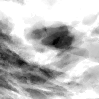
\includegraphics[width=0.13\textwidth]
  {figure/all/dataset_1/proj_roi}

  \raisebox{0.5em}{\fontsize{9}{9}\selectfont
    \rotatebox{90}{Reconstruction}}
  
\includegraphics[width=0.13\textwidth]
  {figure/all/dataset_1/model_coronal}
  
\includegraphics[width=0.13\textwidth]
  {figure/all/dataset_1/model_saggital}
  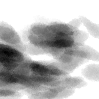
\includegraphics[width=0.13\textwidth]
  {figure/all/dataset_1/proj_roi_inten10}

  {\fontsize{9}{9}\selectfont VOI \#3} \vspace{1mm}

  \raisebox{0.5em}{\fontsize{9}{9}\selectfont \rotatebox{90}{Ground
      truth}}
  
\includegraphics[width=0.13\textwidth]
  {figure/all/dataset_3/roi_coronal}
  
\includegraphics[width=0.13\textwidth]
  {figure/all/dataset_3/roi_saggital}
  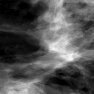
\includegraphics[width=0.13\textwidth]
  {figure/all/dataset_3/proj_roi}

  \raisebox{0.5em}{\fontsize{9}{9}\selectfont
    \rotatebox{90}{Reconstruction}}
  
\includegraphics[width=0.13\textwidth]
  {figure/all/dataset_3/model_coronal}
  
\includegraphics[width=0.13\textwidth]
  {figure/all/dataset_3/model_saggital}
  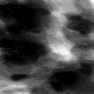
\includegraphics[width=0.13\textwidth]
  {figure/all/dataset_3/proj_roi_inten10}

  {\fontsize{9}{9}\selectfont VOI \#7} \vspace{1mm}

  \raisebox{0.5em}{\fontsize{9}{9}\selectfont \rotatebox{90}{Ground
      truth}}
  
\includegraphics[width=0.13\textwidth]
  {figure/all/dataset_7/roi_coronal}
  
\includegraphics[width=0.13\textwidth]
  {figure/all/dataset_7/roi_saggital}
  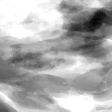
\includegraphics[width=0.13\textwidth]
  {figure/all/dataset_7/proj_roi}

  \raisebox{0.5em}{\fontsize{9}{9}\selectfont
    \rotatebox{90}{Reconstruction}}
  
\includegraphics[width=0.13\textwidth]
  {figure/all/dataset_7/model_coronal}
  
\includegraphics[width=0.13\textwidth]
  {figure/all/dataset_7/model_saggital}
  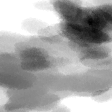
\includegraphics[width=0.13\textwidth]
  {figure/all/dataset_7/proj_roi_inten10}

  {\fontsize{9}{9}\selectfont VOI \#11} \vspace{1mm}

  \raisebox{0.5em}{\fontsize{9}{9}\selectfont \rotatebox{90}{Ground
      truth}}
  
\includegraphics[width=0.13\textwidth]
  {figure/all/dataset_11/roi_coronal}
  
\includegraphics[width=0.13\textwidth]
  {figure/all/dataset_11/roi_saggital}
  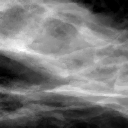
\includegraphics[width=0.13\textwidth]
  {figure/all/dataset_11/proj_roi}

  \raisebox{0.5em}{\fontsize{9}{9}\selectfont
    \rotatebox{90}{Reconstruction}}
  \stackon{\fontsize{9}{9}\selectfont
    Coronal}{
\includegraphics[width=0.13\textwidth]
    {figure/all/dataset_11/model_coronal}}
  \stackon{\fontsize{9}{9}\selectfont
    Saggital}{
\includegraphics[width=0.13\textwidth]
    {figure/all/dataset_11/model_saggital}}
  \stackon{\fontsize{9}{9}\selectfont
    Projection}{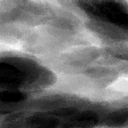
\includegraphics[width=0.13\textwidth]
    {figure/all/dataset_11/proj_roi_inten10}}

  \caption{From left to right, the three columns on the left shows:
    coronal slices through four segmented clinical bCT VOIs, saggital
    slices through the same bCT VOIs and projections of the same bCT
    VOIs. From left to right, the three columns on the right shows:
    coronal slices through the reconstructed VOIs, saggital slices
    through the reconstructed VOIs and projections of the
    reconstructed VOIs. The sizes of the VOIs are \SI{3.5}{\cm}
    $\times$ \SI{3.5}{\cm} $\times$ \SI{3.5}{\cm}. Reconstructed VOIs
    are binary volumes with the same size and resolution as their
    corresponding segmented clinical bCT VOIs. They were created by
    voxelizing the reconstructed ellipsoids from the MBDS algorithm
    and assigning value 0 to the ellipsoid interior. Projections
    images were obtained by averaging the VOIs in the direction
    perpendicular to the transverse plane. The distribution and
    morphology of the medium scale fibroglandular and inter-glandular
    adipose tissue in reconstructed VOIs agree fairly well with the
    original segmented clinical bCT VOIs}
  \label{fig:bct-datasets-recon}

\end{figure}

To demonstrate the convergence of the MBDS algorithm,
Figure~\ref{fig:conv-mbds} shows the decrease of the energy with the
increasing number of iterations for the four examples of bCT
VOIs. From this figure we can see that the convergence was reached
after about 7500 iterations for all the cases. Similar results were
obtained for other investigated bCT VOIs.

\begin{figure}[!htb]
  \centering
  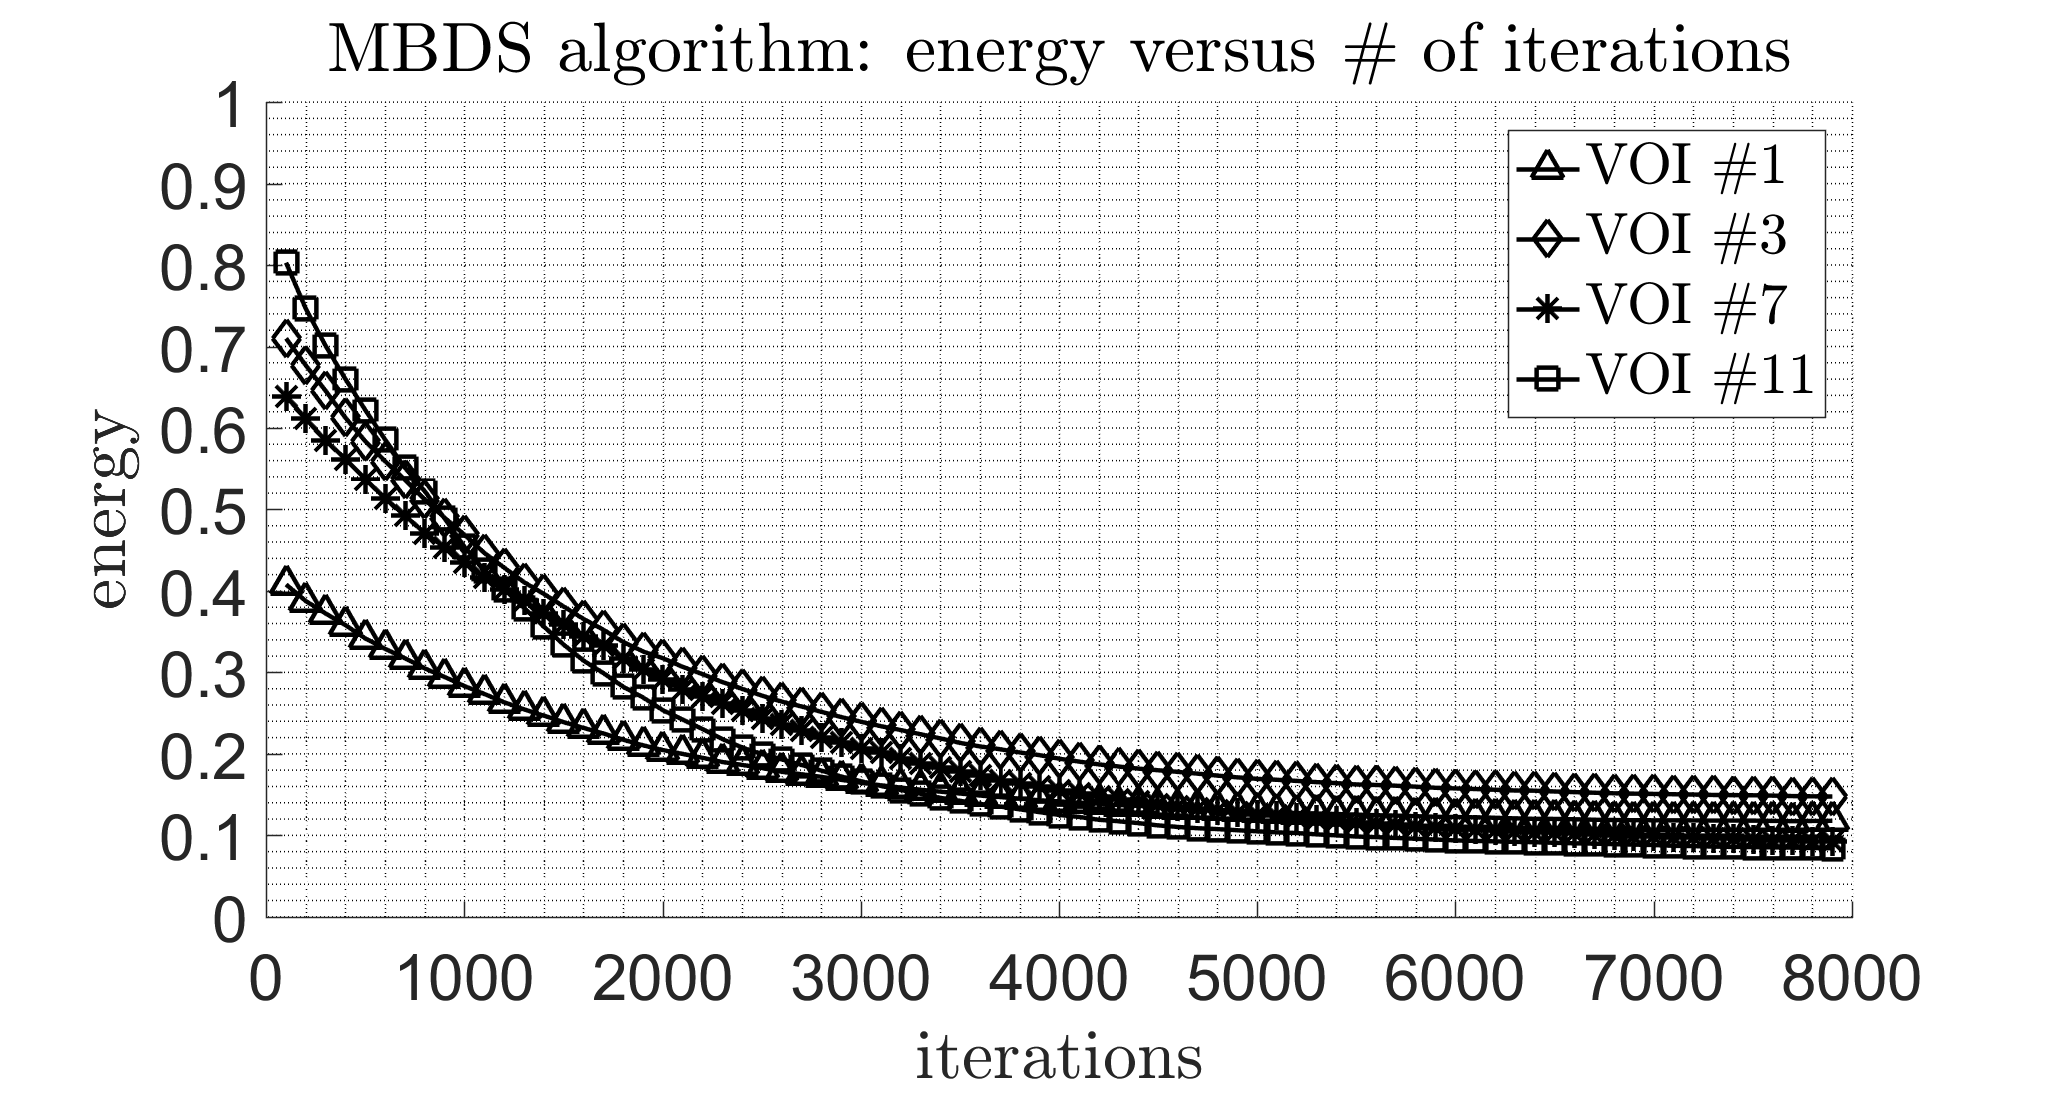
\includegraphics[width=0.5\textwidth]
  {figure/convergence_mbds}
  \caption{Illustration of the energy defined in~\eqref{mpp-energy} as
    a function of the number of iterations in the MBDS algorithm. The
    illustration considers the four examples of segmented clinical bCT
    VOIs shown in Figure~\ref{fig:bct-datasets-recon}. The convergence
    of the MBDS algorithm was reached after about 7500 iterations for
    all the cases.}
  \label{fig:conv-mbds}
\end{figure}

\subsection{Inference step}
\label{chap4-sec4-sub2:result-infer-step}

We first demonstrate the analysis of empirical PCFs estimated from the
reconstructed ellipsoid centers for all selected bCT VOIS using
methodologies described in
Section~\ref{chap5-sec3-sub2:infer-step:-fitt}.

\begin{figure}[!htb]
  \centering

  \captionsetup[subfloat]{labelformat=empty,position=top}

  \subfloat[VOI \#5]{\includegraphics[width=0.25\textwidth]%
    {figure/all/dataset_5/pcf_new}}%
  \subfloat[VOI \#12]{\includegraphics[width=0.25\textwidth]%
    {figure/all/dataset_12/pcf_new}}%

  \subfloat[VOI \#15]{\includegraphics[width=0.25\textwidth]%
    {figure/all/dataset_15/pcf_new}}%
  \subfloat[VOI \#16] {\includegraphics[width=0.25\textwidth]%
    {figure/all/dataset_16/pcf_new}}%

  \caption{Comparison of the empirical PCFs estimated from the
    reconstructed ellipsoid centers for four bCT VOIs (\#5, \#12 \#15
    and \#16) and the theoretical Poisson PCFs. Dashed lines are the
    empirical PCFs estimated from the reconstructed ellipsoid
    centers. Solid lines are theoretical Poisson PCFs. Gray surfaces
    are the envelopes of the Poisson PCFs generated using the method
    described in Section~\ref{chap5-sec3-sub2:infer-step:-fitt}. Based
    on the envelope test described in
    Section~\ref{chap5-sec3-sub2:infer-step:-fitt}, the Poisson
    null-hypothesis can not be rejected at any interpoint distance.}

  % \caption{Example of the analysis of the empirically estimated PCFs
  % for bCT VOIs \#5, \#12 \#15 and \#16. Each figure demonstrates:
  % the estimates of the PCF of the ellipsoid centers reconstructed
  % from the bCT VOIs (dashed line); The theoretical PCF of the
  % Poisson point process (solid line); The envelope of the Poisson
  % point process PCF created using method described in
  % Section~\ref{chap5-sec3-sub2:infer-step:-fitt} (gray
  % surfaces). For the four demonstrated cases, the Poisson
  % null-hypothesis can not be reject at any interpoint distance,
  % based on the envelope test described in
  % Section~\ref{chap5-sec3-sub2:infer-step:-fitt}.}
  \label{fig:pcf-est-non-reject}
\end{figure}

Our analysis shows that, among the 16 selected bCT VOIs, there are
four cases where the Poisson null-hypothesis can not be
rejected. These four case were VOI \#5, \#12 \#15 and
\#16. Figure~\ref{fig:pcf-est-non-reject} compares the empirical PCFs
estimated from the reconstructed ellipsoid centers for these four bCT
VOIs and the theoretical Poisson PCFs. The envelopes of the Poisson
PCFs generated using the method described in
Section~\ref{chap5-sec3-sub2:infer-step:-fitt} are also shown. Based
on the envelope test described in
Section~\ref{chap4-sec3-sub2sub1:ellipsoid-centers}, the Poisson
null-hypothesis can not be rejected at any interpoint distance. Due to
this finding, the VOI \#5, \#12 \#15 and \#16 were left out for the
follow-up study since they represented a much smaller population among
all bCT VOIs.

% Their empirically estimated PCFs are shown in
% Figure~\ref{fig:pcf-est-non-reject}. Theoretical Poisson PCF (solid
% line) and the Poisson envelopes (gray surfaces) generated using
% method described in
% Section~\ref{chap4-sec4-sub2sub1:distr-reconstr-ellip} are also
% shown. From Figure~\ref{fig:pcf-est-non-reject} we can see that, for
% the demonstrated four cases, the Poisson null-hypothesis can not be
% reject at any interpoint distance, based on the two-sided Monte
% Carlo tests described in
% Section~\ref{chap4-sec3-sub2sub1:ellipsoid-centers}. Due to this
% finding, the VOI \#5, \#12 \#15 and \#16 were left out for the
% follow-up study since they represented a much smaller population
% among all bCT VOIs.

Figure~\ref{fig:pcf-est} compares the empirical PCFs estimated from
the reconstructed ellipsoid centers for the four bCT VOIs shown in
Figure~\ref{fig:bct-datasets-recon} and the theoretical Poisson
PCFs. The envelopes of the Poisson PCFs generated using the method
described in Section~\ref{chap5-sec3-sub2:infer-step:-fitt} are also
shown. Figure~\ref{fig:pcf-est} indicates that the empirical PCFs
estimated from the reconstructed ellipsoid centers of the four VOIs
exhibit a clustering effect. This can be seen if we look at the
interpoint distance $r = $ \SI{3}{\mm} emphasized in
Figure~\ref{fig:pcf-est}. The envelope test rejects the
null-hypothesis for all demonstrated VOIs at $r = $ \SI{3}{\mm}. The
same clustering effect was found for all other investigated bCT VOIs.

\begin{figure}[!htb]
  \centering

  \captionsetup[subfloat]{labelformat=empty,position=top}

  \subfloat[{VOI \#1}]{\includegraphics[width=0.25\textwidth]%
    {figure/all/dataset_1/pcf_new}}%
  \subfloat[{VOI \#3}]{\includegraphics[width=0.25\textwidth]%
    {figure/all/dataset_3/pcf_new}}%

  \subfloat[{VOI \#7}]{\includegraphics[width=0.25\textwidth]%
    {figure/all/dataset_7/pcf_new}}%
  \subfloat[{VOI \#11}] {\includegraphics[width=0.25\textwidth]%
    {figure/all/dataset_11/pcf_new}}%

  \caption{Comparison of the empirical PCFs estimated from the
    reconstructed ellipsoid centers for the four bCT VOIs shown in
    Figure~\ref{fig:bct-datasets-recon} and the theoretical Poisson
    PCFs. Dashed lines are the empirical PCFs estimated from the
    reconstructed ellipsoid centers. Solid lines are theoretical PCFs
    of the Poisson point processes. Gray surfaces are the envelopes of
    the Poisson PCFs generated using the method described in
    Section~\ref{chap5-sec3-sub2:infer-step:-fitt}. The envelope test
    rejects the Poisson null-hypothesis for all four VOIs at
    interpoint distance $r = $ \SI{3}{\mm}.}

  % \caption{Example of the analysis of the empirically estimated PCFs
  % for the four examples of bCT VOIs demonstrated in
  % Figure~\ref{fig:bct-datasets-recon}. Each figure demonstrates: the
  % estimates of the PCF of the ellipsoid centers reconstructed from
  % the bCT VOIs (dashed line); The theoretical PCF of the Poisson
  % point process (solid line); The envelope of the Poisson point
  % process PCF created using method described in
  % Section~\ref{chap5-sec3-sub2:infer-step:-fitt} (gray
  % surfaces). From the envelope test described in
  % Section~\ref{chap5-sec3-sub2:infer-step:-fitt}, the Poisson
  % null-hypothesis are rejected for all four cases at interpoint
  % distance $r = $ \SI{3}{\mm}.}
  \label{fig:pcf-est}
\end{figure}

\subsubsection*{Parameters of the 3D Mat\'ern cluster process}
\label{chap4-sec4-sub2sub1:distr-reconstr-ellip}

As discussed in Section~\ref{chap4-sec3-sub2sub1:ellipsoid-centers}, a
3D Mat\'ern cluster process was fitted to each set of reconstructed
ellipsoid centers using the MCE
method. Table~\ref{tab:matern-fit-params} lists the fitted Mat\'ern
cluster process parameters $\hat{\kappa}$, $\hat{\lambda_0}$ and
$\hat{R}$ for ellipsoid centers reconstructed from all bCT VOIs
(excluding VOI \#5, \#12, \#15 and \#16).

Figure~\ref{fig:matern-pcf-fit} compares the empirical PCFs estimated
from the reconstructed ellipsoid centers for the four bCT VOIs shown
in Figure~\ref{fig:bct-datasets-recon} and the theoretical PCFs of the
Mat\'ern cluster processes fitted to the same VOIs. The PCF envelopes
of the fitted Mat\'ern cluster processes were also generated using the
method described in Section~\ref{chap5-sec3-sub2:infer-step:-fitt},
but with the fitted Mat\'ern cluster process as the null hypothesis
model. It can be seen that for all VOIs, the the empirically estimated
PCFs fall inside the envelopes at all interpoint distances. Based on
this, we conclude that the fits are fairly good.

% Figure~\ref{fig:matern-pcf-fit} illustrates the PCFs of the fitted
% Mat\'ern cluster processes. Envelopes of the PCFs of the fitted
% Mat\'ern cluster processes were also generated, using the same
% method as for the Poisson point process described in
% Section~\ref{chap4-sec4-sub2sub1:distr-reconstr-ellip}. It can be
% seen that for all VOIs, the the empirically estimated PCFs fall
% inside the Mat\'{e}rn cluster process envelopes at all considered
% interpoint distances. Based on this, we conclude that the fits are
% fairly good.

\begin{figure}[!htb]
  \centering

  \captionsetup[subfloat]{labelformat=empty,position=top}

  \subfloat[VOI \#1]{\includegraphics[width=0.25\textwidth]%
    {figure/all/dataset_1/fit_pcf_matern}}%
  \subfloat[VOI \#3] {\includegraphics[width=0.25\textwidth]%
    {figure/all/dataset_3/fit_pcf_matern}}%

  \subfloat[VOI \#7]{\includegraphics[width=0.25\textwidth]%
    {figure/all/dataset_7/fit_pcf_matern}}%
  \subfloat[VOI \#11]{\includegraphics[width=0.25\textwidth]%
    {figure/all/dataset_11/fit_pcf_matern}}%

  \caption{Comparison of the empirical PCFs estimated from the
    reconstructed ellipsoid centers for the four bCT VOIs shown in
    Figure~\ref{fig:bct-datasets-recon} and the theoretical PCFs of
    the Mat\'ern cluster processes fitted to the same VOIs. Dashed
    lines are the empirical PCFs estimated from the reconstructed
    ellipsoid centers of the four VOIs. Solid lines are theoretical
    PCFs of the Mat\'ern cluster processes fitted to the four
    VOIs. Gray surfaces are the envelopes of the PCFs of the fitted
    Mat\'ern cluster processes generated using the method described in
    Section~\ref{chap5-sec3-sub2:infer-step:-fitt}. The empirical PCFs
    fall inside the envelopes at all interpoint distances.}
  \label{fig:matern-pcf-fit}
\end{figure}

\begin{table}[!htb]
  \begin{center}
    \begin{tabular}{ m{1.3cm} m{1.5cm} m{1.5cm} m{1.5cm} }
      \toprule

      \centering{\textbf{VOI}}
      & \centering{$\hat{\kappa}$}
      & \centering{$\hat{\lambda_0}$}
      & \centering{$\hat{R}$}
        \tabularnewline%\\

      \cmidrule(lr){1-1} \cmidrule(lr){2-2}
      \cmidrule(lr){3-3} \cmidrule(lr){4-4}

      \centering{\# 1}
      & \centering{4.237e-04}
      & \centering{2.812e-02}
      & \centering{4.221}
        \tabularnewline%\\

        % \centering{\# 2}
        % & \centering{4.719e-02}
        % & \centering{4.331e-02}
        % & \centering{1.218}
        % \tabularnewline%\\

      \centering{\# 3}
      & \centering{3.245e-03}
      & \centering{5.985e-03}
      & \centering{5.988}
        \tabularnewline%\\

        % \centering{\# 4}
        % & \centering{1.014e-04}
        % & \centering{1.515e-02}
        % & \centering{10.408}
        % \tabularnewline%\\

        % \centering{\# 6}
        % & \centering{5.652e-04}
        % & \centering{1.185e-02}
        % & \centering{6.980}
        % \tabularnewline%\\

      \centering{\# 7}
      & \centering{2.876e-04}
      & \centering{3.092e-02}
      & \centering{5.827}
        \tabularnewline%\\

        % \centering{\# 8}
        % & \centering{1.102e-03}
        % & \centering{1.787e-02}
        % & \centering{5.150}
        % \tabularnewline%\\

        % \centering{\# 9}
        % & \centering{1.752e-03}
        % & \centering{1.836e-02}
        % & \centering{4.467}
        % \tabularnewline%\\

        % \centering{\# 10}
        % & \centering{1.374e-02}
        % & \centering{6.429e-03}
        % & \centering{3.643}
        % \tabularnewline%\\

      \centering{\# 11}
      & \centering{3.405e-03}
      & \centering{1.923e-02}
      & \centering{3.853}
        \tabularnewline%\\

        % \centering{\# 13}
        % & \centering{8.206e-04}
        % & \centering{1.380e-02}
        % & \centering{6.608}
        % \tabularnewline%\\

        % \centering{\# 14}
        % & \centering{6.643e-04}
        % & \centering{5.720e-03}
        % & \centering{9.993}
        % \tabularnewline%\\

      \bottomrule

    \end{tabular}
    \caption{Fitted Mat\'ern cluster process parameters for the four
      bCT VOIs shown in Figure~\ref{fig:bct-datasets-recon}.}
    \label{tab:matern-fit-params}
  \end{center}
\end{table}

\subsubsection*{The mark distribution}
\label{chap4-sec4-sub2sub2:distr-semi-princ}

Figure~\ref{fig:ellip-axes-distr} shows the histograms of the half
lengths $L_a$, $L_b$ and $L_c$ of the reconstructed ellipsoids for the
four bCT VOIs shown in Figure~\ref{fig:bct-datasets-recon}. The
empirical mean $\hat{\mu}$ and standard deviation $\hat{\sigma}$, as
well as the $p_1$ and $p_2$ values of the Kolmogorov-Smirnov tests
(described in Section~\ref{chap5-sec3-sub2:infer-step:-fitt}) for each
half length are shown under the histograms.

According to the $p_1$ values, $L_a$, $L_b$ and $L_c$ remain to be
Gaussian distributed for all cases at significance level 5\%. However,
according to the $p_2$ values the distributions of $L_a$, $L_b$ and
$L_c$ deviate significantly from the proposal distrbutions $f_{L_a}$,
$f_{L_b}$ and $f_{L_c}$ respectively, for all cases at the same
significance level.

Figure~\ref{fig:ellip-tilts-distr} shows the histograms of the tilts
angles $\delta\phi_x$, $\delta\phi_y$ and $\delta\phi_z$ of the
reconstructed ellipsoids for the four bCT VOIs shown in
Figure~\ref{fig:bct-datasets-recon}. The empirical minimum and maximum
for $\delta\phi_x$, the empirical mean $\hat{\mu}$ and standard
deviation $\hat{\sigma}$ for $\delta\phi_y$ and $\delta\phi_z$, as
well as the $p_1$ and $p_2$ values of the Kolmogorov-Smirnov tests
(described in Section~\ref{chap5-sec3-sub2:infer-step:-fitt}) for each
tilt angle are shown under the histograms.

% The empirical statistics for each tilt angle are shown under each
% sub-figure. The $p_1$ and $p_2$ values of the Kolmogorov-Smirnov
% tests described in Section~\ref{chap5-sec3-sub2:infer-step:-fitt}
% are also shown.

% According to the $p_1$ and $p_2$ values, the hypothesis that
% $\delta\phi_x$ follows the uniform distribution
% $\mathcal{U}(-\frac{\pi}{2}, \frac{\pi}{2})$ can not be rejected at
% significance level 5\% for all cases.

According to the $p_1$ and $p_2$ values for $\delta\phi_x$, the
distribution of $\delta\phi_x$ does not deviate significantly from the
uniform distribution $\mathcal{U}(-\frac{\pi}{2}, \frac{\pi}{2})$ for
all cases at significance level 5\%. According to the $p_1$ values for
$\delta\phi_y$, $\delta\phi_y$ remains to be Gaussian distributed in
three of the four cases at significance level 5\%. However, according
to $p_2$ values for $\delta\phi_y$, the distribution of $\delta\phi_y$
deviates significantly from the proposal distribution
$f_{\delta{\phi_x}}$ in three of the four cases at significance level
5\%. According to the $p_1$ values for $\delta\phi_z$, $\delta\phi_z$
remains to be Gaussian distributed in two of the four cases at
significance level 5\%. However, according to the $p_2$ values for
$\delta\phi_z$, the distribution of $\delta\phi_z$ deviates
significantly from the proposal distribution $f_{\delta{\phi_x}}$ for
all cases at significance level 5\%. Similar observations were
obtained for all other investigated bCT VOIs.

% Regarding the distribution of $\delta\phi_y$, according to the $p_1$
% values in three of the four cases the Gaussian hypothesis can not be
% rejected at significance level 5\%. However, according to the $p_2$
% values in three of the four cases the null-hypothesis that
% $\delta\phi_y$ follows the proposal distribution
% $f_{\delta{\phi_x}}$ is rejected at significance level 5\%.

% For $\delta\phi_z$, $p_1$ seems to suggest that in half of the four
% cases, the Gaussian distribution can not be rejected at significance
% level 5\%. And finally $p_2$ suggest that the null-hypothesis that
% $\delta\phi_z$ follows the proposal distribution
% $f_{\delta{\phi_z}}$ should all be rejected at significance level
% 5\%.

% Similar observations regarding $\delta\phi_x$ were obtained for the
% rest of the cases not shown in Figure~\ref{fig:ellip-axes-distr}.

% For $\delta\phi_x$ and $\delta\phi_y$, the two Kolmogorov-Smirnov
% tests showed different results for different input VOI.  In three
% out of the four demonstrated cases, the null-hypothesis of the first
% tests for $\delta\phi_y$ can not be rejected at significance level
% 5\%, according to the $p_1$ values.

% However, in the rejected cases, there are 2 cases where the
% hypothesis that $\delta\phi_y$ is Gaussian distributed following
% $f_{\delta{\phi_y}}$ can not be rejected, according to the $p_2$
% values. For the rest of the three VOIs,

% This means that at significance level 5\%, in 66.7\% (8 out of 12)
% of the cases, the hypothesis that $\delta\phi_y$ is Gaussian
% distributed can not be rejected.

% According to the $p_1$ values, in 66.7\% (8 out of 12) of the cases,
% the hypothesis that $\delta\phi_x$ follows uniform distribution can
% not be rejected at significance level 5\%. For these cases, the
% hypothesis that $\delta\phi_x$ is uniformly distributed following
% $f_{\delta{\phi_x}}$ also can not be rejected at the same
% significance level, according to the $p_2$ values.

% In 50\% (6 out of 12) of the cases, the null-hypothesis of the first
% tests for $\delta\phi_y$ can not be rejected at significance level
% 5\%, according to the $p_1$ values. However, in the rejected cases,
% there are 2 cases where the hypothesis that $\delta\phi_y$ is
% Gaussian distributed following $f_{\delta{\phi_y}}$ can not be
% rejected, according to the $p_2$ values. This means that at
% significance level 5\%, in 66.7\% (8 out of 12) of the cases, the
% hypothesis that $\delta\phi_y$ is Gaussian distributed can not be
% rejected.

% Finally regarding $\delta\phi_z$, using analysis similar to that for
% $\delta\phi_y$, we conclude that at significance level 5\%, in
% 41.67\% (5 out of 12) of the cases, the hypothesis that
% $\delta\phi_z$ is Gaussian distributed can not be rejected.

\begin{figure}[!htb]
  \centering

  \captionsetup[subfloat]{labelformat=empty,position=top}

  \subfloat[VOI \#1]{\includegraphics[width=0.25\textwidth]%
    {figure/all/dataset_1/axes_distr_new}}%
  \subfloat[VOI \#3]{\includegraphics[width=0.25\textwidth]%
    {figure/all/dataset_3/axes_distr_new}}%

  \subfloat[VOI \#7]{\includegraphics[width=0.25\textwidth]%
    {figure/all/dataset_7/axes_distr_new}}%
  \subfloat[VOI \#11]{\includegraphics[width=0.25\textwidth]%
    {figure/all/dataset_11/axes_distr_new}}%

  \caption{Histograms of the half lengths $L_a$, $L_b$ and $L_c$ of
    reconstructed ellipsoids for the four bCT VOIs shown in
    Figure~\ref{fig:bct-datasets-recon}. For each half length,
    $\hat{\mu}$ and $\hat{\sigma}$ refer respectively to their
    empirical mean and standard deviation. For each half length, $p_1$
    and $p_2$ refer to the $p$-values of the two Kolmogorov-Smirnov
    tests described in
    Section~\ref{chap5-sec3-sub2:infer-step:-fitt}.}
  \label{fig:ellip-axes-distr}
\end{figure}

\begin{figure}[!htb]
  \centering

  \captionsetup[subfloat]{labelformat=empty,position=top}

  \subfloat[VOI \#1]{\includegraphics[width=0.25\textwidth]%
    {figure/all/dataset_1/tilts_distr_new}}%
  \subfloat[VOI \#3]{\includegraphics[width=0.25\textwidth]%
    {figure/all/dataset_3/tilts_distr_new}}%

  \subfloat[VOI \#7]{\includegraphics[width=0.25\textwidth]%
    {figure/all/dataset_7/tilts_distr_new}}%
  \subfloat[VOI \#11]{\includegraphics[width=0.25\textwidth]%
    {figure/all/dataset_11/tilts_distr_new}}%

  \caption{Histograms of the tilt angles $\delta\phi_x$,
    $\delta\phi_y$ and $\delta\phi_z$ of reconstructed ellipsoids from
    the four bCT VOIs shown in Figure~\ref{fig:bct-datasets-recon}.
    For $\delta\phi_x$, $\min$ and $\max$ refer respectively to its
    empirical minimum and maximum. For $\delta\phi_y$ and
    $\delta\phi_z$, $\hat{\mu}$ and $\hat{\sigma}$ refer respectively
    to their empirical mean and standard deviation. For each tilt
    angle, $p_1$ and $p_2$ refer to the $p$-values of the two
    Kolmogorov-Smirnov tests described in
    Section~\ref{chap5-sec3-sub2:infer-step:-fitt}.}
  \label{fig:ellip-tilts-distr}
\end{figure}

Based on these analyses, we proposed to model the distribution
$\mathbf{P}^{\boldsymbol{\theta}}$ of the marks
$\boldsymbol{\theta} = \left( L_a, L_b, L_c, \delta\phi_x,
  \delta\phi_y, \delta\phi_z \right)$ as independent densities
$p_{L_a}$, $p_{L_b}$, $p_{L_c}$, $p_{\delta\phi_x}$,
$p_{\delta\phi_y}$ and $p_{\delta\phi_z}$ respectively. These
densities are specified as follows.

The distribution of the half lengths of the ellipsoids, namely
$p_{L_a}$, $p_{L_b}$ and $p_{L_c}$ were all modeled as Gaussian
distributions. The mean and standard deviation of $p_{L_a}$, $p_{L_b}$
and $p_{L_c}$ were determined by the values empirically measured from
the ellipsoids reconstructed from the clinical bCT VOIs. The mean and
standard deviation values were specified in
Figure~\ref{fig:ellip-axes-distr}.

The distribution of the tilt angles $\delta\phi_x$, $p_{\delta\phi_x}$
was model as the uniform distribution
$\mathcal{U} \left( -\frac{\pi}{2}, \frac{\pi}{2} \right)$, as
suggested by its empirical distribution demonstrated in the previous
section.

The distributions $p_{\delta\phi_y}$ and $p_{\delta\phi_z}$ were
modeled as Gaussian distributions. Despite the fact that in some of
the cases, the Gaussian hypothesis was rejected by the
Kolmogorov-Smirnov tests, as mentioned in the previous section, in
other majority of the cases the Gaussian hypothesis could not be
rejected. Visual inspection of the histograms of $p_{\delta\phi_y}$
and $p_{\delta\phi_z}$ also suggests that the Gaussian distribution
might still be a fairly reasonable choice. Similar to the half
lengths, the mean and standard deviation of $p_{\delta\phi_y}$ and
$p_{\delta\phi_z}$ are determined by the empirical estimates.

We finally obtained twelve new sets of medium scale parameters for the
3D solid breast texture model from the twelve input segmented bCT
VOIs. Table~\ref{tab:summary-inferred-params} lists the fitted medium
scale parameters for the four bCT VOIs shown in
Figure~\ref{fig:bct-datasets-recon}. Parameters fitted using the other
eight bCT VOIs can be found in
Appendix~\ref{app2:addit-results-chapt}.

\begin{table}[!htb]
  \begin{center}
    \begin{tabular}{ m{1cm} m{2cm} m{2cm} m{2cm} }
      \toprule

      \centering{\textbf{VOI}}
      & \centering{\textbf{$\boldsymbol{\Phi}_s$ (Mat\'ern cluster
        process)}}
      & \centering{$L_a$, $L_b$, $L_c$ (in $mm$)}
      & \centering{$\delta_{\phi_x}$,
        $\delta_{\phi_y}$, $\delta_{\phi_z}$ (in radian)}
        \tabularnewline%\\

      \cmidrule(lr){1-1} \cmidrule(lr){2-2}
      \cmidrule(lr){3-3} \cmidrule(lr){4-4}

      \centering{\#1}
      & \centering{$\kappa = 4.237e-04$, $\lambda_0 = 2.812e-02$, $R =
        4.221$}
      & \centering{$f_{L_a} = \mathcal{N}(5.48, 1.34)$,
        $p_{L_b} = \mathcal{N}(2.72, 0.55)$,
        $p_{L_c} = \mathcal{N}(1.90, 0.48)$}
      & $p_{\delta_{\phi_x}} = \mathcal{U}(-\frac{\pi}{2},
        \frac{\pi}{2})$,

        $p_{\delta_{\phi_y}} = \mathcal{N}(-0.05, 0.35)$,

        $p_{\delta_{\phi_z}} = \mathcal{N}(-0.04, 0.53)$
        \tabularnewline%\\

      \cmidrule(lr){1-1} \cmidrule(lr){2-2}
      \cmidrule(lr){3-3} \cmidrule(lr){4-4}

      \centering{\#3}
      & \centering{$\kappa = 3.245e-03$, $\lambda_0 = 5.985e-03$, $R =
        5.988$}
      & \centering{$p_{L_a} = \mathcal{N}(6.21, 1.41)$,
        $p_{L_b} = \mathcal{N}(2.77, 0.58)$,
        $p_{L_c} = \mathcal{N}(2.10, 0.57)$}
      & $p_{\delta_{\phi_x}} = \mathcal{U}(-\frac{\pi}{2},
        \frac{\pi}{2})$,

        $p_{\delta_{\phi_y}} = \mathcal{N}(-0.09, 0.4)$,

        $p_{\delta_{\phi_z}} = \mathcal{N}(0, 0.26)$
        \tabularnewline%\\

      \cmidrule(lr){1-1} \cmidrule(lr){2-2}
      \cmidrule(lr){3-3} \cmidrule(lr){4-4}

      \centering{\#7}
      & \centering{$\kappa = 2.876e-04$, $\lambda_0 = 3.092e-02$,
        $R =
        5.827$}
      & \centering{$p_{L_a} = \mathcal{N}(5.88, 1.44)$,
        $p_{L_b} = \mathcal{N}(2.75, 0.56)$,
        $p_{L_c} = \mathcal{N}(2.03, 0.52)$}
      & $p_{\delta_{\phi_x}} = \mathcal{U}(-\frac{\pi}{2},
        \frac{\pi}{2})$,

        $p_{\delta_{\phi_y}} = \mathcal{N}(-0.15, 0.38)$,

        $p_{\delta_{\phi_z}} = \mathcal{N}(0.01, 0.5)$
        \tabularnewline%\\

      \cmidrule(lr){1-1} \cmidrule(lr){2-2}
      \cmidrule(lr){3-3} \cmidrule(lr){4-4}

      \centering{\#11}
      & \centering{$\kappa = 3.405e-03$, $\lambda_0 = 1.923e-02$,
        $R =
        3.853$}
      & \centering{$p_{L_a} = \mathcal{N}(6.06, 1.39)$,
        $p_{L_b} = \mathcal{N}(2.79, 0.56)$,
        $p_{L_c} = \mathcal{N}(2.10, 0.54)$}
      & $p_{\delta_{\phi_x}} = \mathcal{U}(-\frac{\pi}{2},
        \frac{\pi}{2})$,

        $p_{\delta_{\phi_y}} = \mathcal{N}(-0.28, 0.47)$,

        $p_{\delta_{\phi_z}} = \mathcal{N}(-0.01, 0.43)$
        \tabularnewline%\\

      \bottomrule

    \end{tabular}

    \caption{Medium scale parameters for the 3D stochastic breast
      texture model fitted from the four bCT VOIs shown in
      Figure~\ref{fig:bct-datasets-recon}.}
    \label{tab:summary-inferred-params}
  \end{center}
\end{table}


\subsection{Simulations using fitted medium scale texture model
  parameters}
\label{chap04-sec4-sub3:simulations}

As a preliminary validation of the fitted medium scale texture model
parameters, a simulation experiment in analogy to
Section~\ref{chap4-sec3:prelim-sims} was conducted.

Four texture volumes were simulated using the four sets of medium
scale parameters listed in
Table~\ref{tab:summary-inferred-params}. The small scale textures in
these volumes were also simulated using parameters listed in
Table~\ref{tab:emp-params-adj}. The nipple position and the voxel size
for each volume were set to be the same as in the corresponding ground
truth bCT VOI. Mammograms and DBT projection images were simulated by
virtually projecting the texture volumes using the previously
described breast x-ray imaging simulator \cite{milioni2014low}, with
the same adjustment as described in
Section~\ref{chap4-sec1-sub2:analys-segm-bct}. Mechanical breast
texture deformation to mimic breast compression was not modeled for
neither mammography and DBT simulation acquisitions. Projection images
were processed by the \texttt{ASiR-DBT} 3D reconstruction algorithm
(version 1.3.4, GE Healthcare, Buc, France) to obtain DBT
reconstructed slices with \SI{1}{\mm} slice thickness.

Figure~\ref{fig:fit-params-sims} shows examples of \SI{3.5}{\cm}
$\times$ \SI{3.5}{\cm} slices through volumes simulated from the 3D
breast texture model with the four sets of medium scale parameters
listed in Table~\ref{tab:summary-inferred-params}, as well as
mammographic projections and DBT reconstructed slices simulated from
these volumes. Images simulated with the other eight sets of
parameters can be found in Appendix~\ref{app2:addit-results-chapt}.

Visual inspection of the simulated images indicates high visual
realism compared with the images simulated from segmented clinical bCT
VOIs, shown in Figure~\ref{fig:bct-selected-sims}. Also, compared with
images simulated using the prototype implementation shown in
Figure~\ref{figure:model-imgs}, the new model parameters are capable
of simulating mammographic projections and and DBT reconstructed
slices with a larger morphological variability. These observations
indicate an improvement of the model's realism and morphological
variability compared with the prototype implementation with empirical
parameters proposed in the previous chapter.

\begin{figure}[!htb]
  \centering

  \captionsetup[subfloat]{labelformat=empty}

  \hspace{1mm} \parbox{2.8cm}{\fontsize{9}{9}\selectfont \centering
    Texture volumes slices} \parbox{2.8cm}{\fontsize{9}{9}\selectfont
    \centering Mammographic
    projections} \parbox{2.75cm}{\fontsize{9}{9}\selectfont \centering
    DBT reconstructed slices} \vspace{1mm}

  \raisebox{3em}{\fontsize{9}{9}\selectfont \rotatebox{90}{VOI \#1}}
  
\includegraphics[width=0.15\textwidth]
  {figure/all/dataset_1/sim_vol_small}
  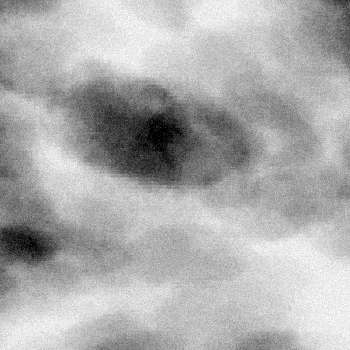
\includegraphics[width=0.15\textwidth]
  {figure/all/dataset_1/sim_proj}
  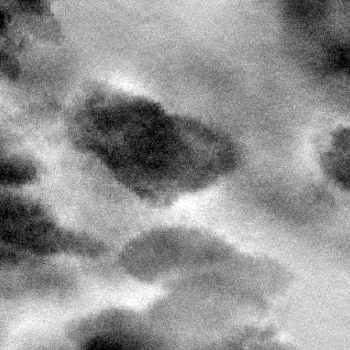
\includegraphics[width=0.15\textwidth]
  {figure/all/dataset_1/sim_recon}

  \raisebox{3em}{\fontsize{9}{9}\selectfont \rotatebox{90}{VOI \#3}}
  
\includegraphics[width=0.15\textwidth]
  {figure/all/dataset_3/sim_vol_small}
  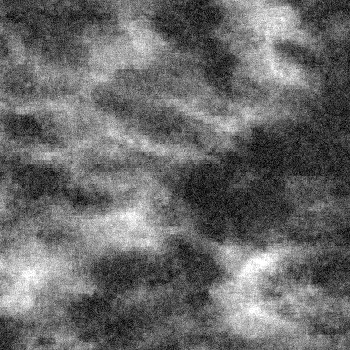
\includegraphics[width=0.15\textwidth]
  {figure/all/dataset_3/sim_proj}
  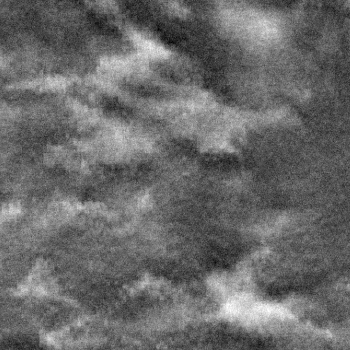
\includegraphics[width=0.15\textwidth]
  {figure/all/dataset_3/sim_recon}

  \raisebox{3em}{\fontsize{9}{9}\selectfont \rotatebox{90}{VOI \#7}}
  
\includegraphics[width=0.15\textwidth]
  {figure/all/dataset_7/sim_vol_small}
  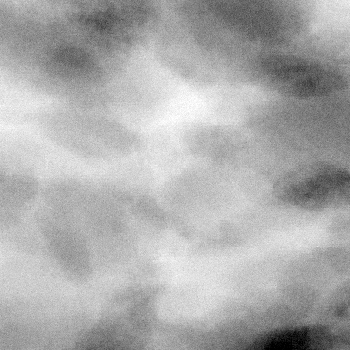
\includegraphics[width=0.15\textwidth]
  {figure/all/dataset_7/sim_proj}
  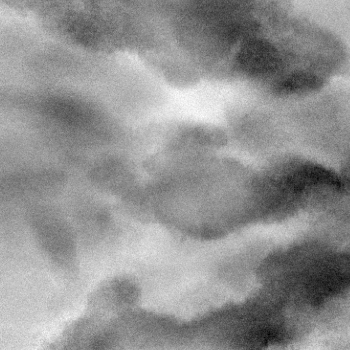
\includegraphics[width=0.15\textwidth]
  {figure/all/dataset_7/sim_recon}

  \raisebox{3em}{\fontsize{9}{9}\selectfont \rotatebox{90}{VOI \#11}}
  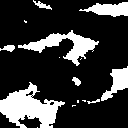
\includegraphics[width=0.15\textwidth]
  {figure/all/dataset_11/sim_vol_small}
  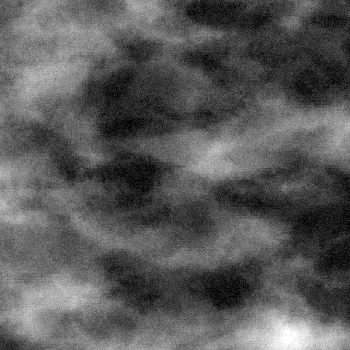
\includegraphics[width=0.15\textwidth]
  {figure/all/dataset_11/sim_proj}
  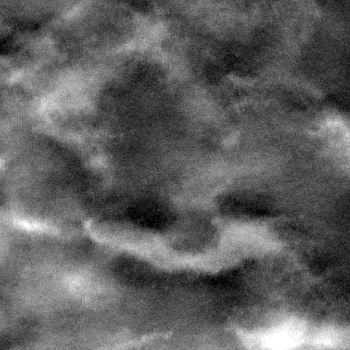
\includegraphics[width=0.15\textwidth]
  {figure/all/dataset_11/sim_recon}

  % \caption{Examples of (\SI{3.5}{\cm})$^2$ ROIs of volume slices,
  % mammographic projections and reconstructed DBT slices simulated
  % using the 3D stochastic breast texture model with the four sets of
  % parameters summarized in Table~\ref{tab:summary-inferred-params}.

  \caption{The first column shows slices through volumes simulated
    from the 3D breast texture model with the four sets of parameters
    listed in Table~\ref{tab:summary-inferred-params}. The second
    column shows mammographic projections simulated from the simulated
    texture volumes. The third column shows DBT reconstructed slices
    simulated from the simulated texture volumes. The sizes of the
    images are \SI{3.5}{\cm} $\times$ \SI{3.5}{\cm}.}
  \label{fig:fit-params-sims}
\end{figure}

\section{Conclusion and discussion}
\label{sec:concl-disc}

In this chapter, we applied a novel methodology based on inference
from reconstruction to automatically and objectively infer the medium
scale 3D breast texture model parameters from \SI{3.5}{\cm} $\times$
\SI{3.5}{\cm} $\times$ \SI{3.5}{\cm} volumes of interest (VOI) of
segmented clinical breast computerized tomography (bCT) reconstructed
datasets.

A multiple births, deaths and shifts (MBDS) algorithm was employed to
first reconstruct a set of random ellipsoids from each ground truth
bCT VOI. Visual inspection of the volumes recreated by voxelizing the
reconstructed ellipsoids shows a fairly good approximation of the
medium scale breast tissue in the original bCT VOIs. A Mat\'{e}rn
cluster process was then fitted to the reconstructed ellipsoid centers
using the minimum contrast method based on the pair correlation
functions (PCF). This introduces a clustering interaction between
ellipsoids to the previous prototype model. Statistical diagnostic
analysis using the PCF suggested a fairly good fit of the
reconstructed ellipsoid centers to the proposed Mat\'{e}rn cluster
process. Distributions of the ellipsoid half lengths and orientations
were finally estimated from their empirical distributions. Twelve sets
of new medium scale model parameters were obtained. Preliminary
evaluation of the 2D and 3D breast images simulated from 3D texture
volumes generated using new parameters shows fairly high visual
realism. The breast tissue variability in new simulated images is
larger than the images simulated using previously proposed prototype
implementation with empirical parameters.

The proposed method has several limitations. First, the impact of the
reconstruction step on the estimated parameters in the inference step
was not investigated. To address this, one possible approach is to
study how the inference result deviates from a ground truth model when
the latter is a known Poisson marked point process. Second, to reduce
the optimization complexity in the inference step, the distribution of
ellipsoid half lengths were estimated independently from the ellipsoid
centers. This may be a simplification compared with the distribution
of inter-glandular adipose compartments in real breasts. The
correlation between the the half lengths and the centers of the
ellipsoids could be further investigated by studying the mark
correlation function of the reconstructed ellipsoids. The statistical
properties of simulated 2D and 3D breast images using inferred medium
scale model parameters were not studied. This should be addressed next
as a further validation of the new models. Also, a formal observer
psycho-physical experiment should be performed to validate the visual
realism of images simulated using the fitted medium scale model
parameters.




% if have a single appendix:
% \appendix[Proof of the Zonklar Equations]
% or
% \appendix % for no appendix heading
% do not use \section anymore after \appendix, only \section* is
% possibly needed

% use appendices with more than one appendix then use \section to
% start each appendix you must declare a \section before using any
% \subsection or using \label (\appendices by itself starts a section
% numbered zero.)
%


\appendices
\section{Proof of the First Zonklar Equation}
Appendix one text goes here.

% you can choose not to have a title for an appendix if you want by
% leaving the argument blank
\section{}
Appendix two text goes here.


% use section* for acknowledgment
\section*{Acknowledgment}


The authors would like to thank...


% Can use something like this to put references on a page by
% themselves when using endfloat and the captionsoff option.
\ifCLASSOPTIONcaptionsoff
\newpage
\fi



% trigger a \newpage just before the given reference number - used to
% balance the columns on the last page adjust value as needed - may
% need to be readjusted if the document is modified later
% \IEEEtriggeratref{8} The "triggered" command can be changed if
% desired: \IEEEtriggercmd{\enlargethispage{-5in}}

% references section

% can use a bibliography generated by BibTeX as a .bbl file BibTeX
% documentation can be easily obtained at:
% http://mirror.ctan.org/biblio/bibtex/contrib/doc/ The IEEEtran
% BibTeX style support page is at:
% http://www.michaelshell.org/tex/ieeetran/bibtex/
% \bibliographystyle{IEEEtran} argument is your BibTeX string
% definitions and bibliography database(s)
% \bibliography{IEEEabrv,../bib/paper}
%
% <OR> manually copy in the resultant .bbl file set second argument
% of \begin to the number of references (used to reserve space for the
%   reference number labels box)

% \begin{thebibliography}{1}

% \bibitem{IEEEhowto:kopka} H.~Kopka and P.~W. Daly, \emph{A Guide to
%     \LaTeX}, 3rd~ed.\hskip 1em plus 0.5em minus 0.4em\relax Harlow,
%   England: Addison-Wesley, 1999.

% \end{thebibliography}

\bibliography{biblio/biblio}
\bibliographystyle{ieeetr}

% biography section
%
% If you have an EPS/PDF photo (graphicx package needed) extra braces
% are needed around the contents of the optional argument to biography
% to prevent the LaTeX parser from getting confused when it sees the
% complicated
% \includegraphics command within an optional argument. (You could
% create your own custom macro containing the \includegraphics command
% to make things simpler here.)
% \begin{IEEEbiography}[{\includegraphics[width=1in,height=1.25in,clip,keepaspectratio]{mshell}}]{Michael
%   Shell}
%   or if you just want to reserve a space for a photo:

\begin{IEEEbiography}{Michael Shell}
  Biography text here.
\end{IEEEbiography}

% if you will not have a photo at all:
\begin{IEEEbiographynophoto}{John Doe}
  Biography text here.
\end{IEEEbiographynophoto}

% insert where needed to balance the two columns on the last page with
% biographies
% \newpage

\begin{IEEEbiographynophoto}{Jane Doe}
  Biography text here.
\end{IEEEbiographynophoto}

% You can push biographies down or up by placing a \vfill before or
% after them. The appropriate use of \vfill depends on what kind of
% text is on the last page and whether or not the columns are being
% equalized.

% \vfill

% Can be used to pull up biographies so that the bottom of the last
% one is flush with the other column.  \enlargethispage{-5in}



% that's all folks
\end{document}



%%% Local Variables:
%%% mode: latex
%%% TeX-master: t
%%% End:
